
\documentclass[preprint,12pt,a4paper]{elsarticle}

\usepackage{lineno}
% \usepackage{hredyperref}
\usepackage{float}
\usepackage{subfig}
\usepackage{color}
\usepackage{soul}
\usepackage{cancel}

% Packages to write pseudo-algorithms %
\usepackage{algorithm}
\usepackage{algorithmic}

\usepackage{cancel}

\usepackage{subfigure} % subfiguras

\usepackage{amsmath,amsthm,amssymb}
\usepackage{xstring}


% Tikz
\usepackage{stanli}
\usepackage[ugly]{units}
% \usetikzlibrary{decorations}
% \usetikzlibrary{arrows}
\usetikzlibrary{plotmarks}

\usetikzlibrary{%
    decorations.pathreplacing,%
    decorations.pathmorphing%
}


\newcommand{\vect}[1]{
  \ensuremath{\mathbf{{#1}}}
}
\newcommand{\tens}[1]{
  \ensuremath{\mathbf{{#1}}}
}
\newcommand{\Matrix}[1]{
  \ensuremath{\mathbf{{#1}}}
}
\newcommand{\Vector}[1]{
  \ensuremath{\mathbf{{#1}}}
}
% Divergence
\newcommand{\Div}[1]{
  \ensuremath{div({#1})}
}
% Gradient
\newcommand\Grad[1]{grad({#1})}
\newcommand\GradS[1]{grad^s({#1})}
\newcommand\GradT[1]{grad^T({#1})}
% Partial derivative
\newcommand{\Deriv}[3][]{
  \ensuremath{\frac{\partial^{#1}{#2}}{ \partial {#3}^{#1} }}
}
% Integral
\newcommand{\Integral}[2]{
  \IfStrEqCase{#1}{
    {2}{\ensuremath{\int_{\varGamma_d}{#2}\ d\varGamma}}
    {3}{\ensuremath{\int_{\varOmega}{#2}\ d\varOmega}}
  }
}

%%%%%%%%%%%%%%%%%%%%%%%%%%%%%%%%%%%%%%%%%%%%%%%%%%%%%%%%%%%%%%%%%%%%
% Init glossaries
\usepackage[acronym]{glossaries}

\makeglossaries

\newglossaryentry{domain}
{
  name=$\varOmega$,
  description={Continuum domain}
}

\newglossaryentry{contour}
{
  name=$\partial\varOmega$,
  description={Boundary of the continuum domain $\varOmega$. Also
    defined as $\Gamma$}
}

\newglossaryentry{dirichlet-boundary}
{
  name=$ \Gamma_d$,
  description={Essential or Dirichlet boundary conditions over $\partial\varOmega$}
}

\newglossaryentry{neumann-boundary}
{
  name=$ \Gamma_n$,
  description={Natural or Nemann boundary conditions over $\partial\varOmega$}
}

\newglossaryentry{rho}
{
  name=$\rho$,
  description={Describes the scalar density field}
}

\newglossaryentry{a}
{
  name=$\vect{a}$,
  description={First order tensor which describes the acceleration field}
}

\newglossaryentry{v}
{
  name=$\vect{v}$,
  description={First order tensor which describes the velocity field}
}

\newglossaryentry{u}
{
  name=$\vect{u}$,
  description={First order tensor which describes the displacement field}
}

\newglossaryentry{x}
{
  name=$\vect{x}$,
  description={First order tensor which describes the global coordinates field}
}

\newglossaryentry{xi}
{
  name=$\vect{\xi}$,
  description={First order tensor which describes the local coordinates field}
}


\newglossaryentry{stress}
{
  name=$\tens{\sigma}$,
  description={Second order tensor which means the Cauchy stress tensor}
}


\newglossaryentry{strain}
{
  name=$\tens{\varepsilon}$,
  description={Second order tensor which means the Cauchy strain tensor}
}


\newglossaryentry{Constitutive}
{
  name=$\tens{D}$,
  description={Four order tensor which means the constitutive response
    of the material}
}


\newglossaryentry{LME-beta}
{
  name=$\beta$,
  description={Regularization or thermalization parameter of the
    LME$_{\beta}$ Pareto set}
}

\newacronym{mpm}{MPM}{Material Point Method}
\newacronym{otm}{OTM}{Optimal Transportation Meshfree}
\newacronym{sph}{SPH}{Smoothed Particle Hydrodynamics}
\newacronym{fem}{FEM}{Finite Element Method}
\newacronym{lme}{LME}{Local Maximum-Entropy}
\newacronym{flip}{FLIP}{Fluid Implicit Particle}
\newacronym{gimp}{GIMP}{Generalized Interpolation Material Point}
\newacronym{igimp}{iGIMP}{Implicit GIMP}
\newacronym{ugimp}{uGIMP}{Uniform GIMP}
\newacronym{ddmp}{DDMP}{Dual Domain Material Point}
\newacronym{ctls}{CTLS}{Conservative Taylor Least Squares}
\newacronym{npc}{NPC}{Newmark Predictor-Corrector}
\newacronym{fe}{FE}{Forward Euler}

% End glossaries
%%%%%%%%%%%%%%%%%%%%%%%%%%%%%%%%%%%%%%%%%%%%%%%%%%%%%%%%%%%%%%%%%%%%

\newcommand{\red}[1]{
  \textcolor{red}{{#1}}
}

\newcommand{\MMP}[1]{
  \textcolor{blue}{{#1}}
}


%%%%%%%%%%%%%%%%%%%%%%%%%%%%%%%%%%%%%%%%%%%%%%%%%%%%%%%%%%%%%%%%%%%%

\modulolinenumbers[5]

\journalname{Computer Methods in Applied Mechanics and Engineering}

%%%%%%%%%%%%%%%%%%%%%%%
%% Elsevier bibliography styles
%%%%%%%%%%%%%%%%%%%%%%%
%% To change the style, put a % in front of the second line of the current style and
%% remove the % from the second line of the style you would like to use.
%%%%%%%%%%%%%%%%%%%%%%%

%% Numbered
%\bibliographystyle{model1-num-names}

%% Numbered without titles
%\bibliographystyle{model1a-num-names}

%% Harvard
%\bibliographystyle{model2-names.bst}\biboptions{authoryear}

%% Vancouver numbered
%\usepackage{numcompress}\bibliographystyle{model3-num-names}

%% Vancouver name/year
%\usepackage{numcompress}\bibliographystyle{model4-names}\biboptions{authoryear}

%% APA style
%\bibliographystyle{model5-names}\biboptions{authoryear}

%% AMA style
%\usepackage{numcompress}\bibliographystyle{model6-num-names}

%% `Elsevier LaTeX' style
\bibliographystyle{elsarticle-num}
%%%%%%%%%%%%%%%%%%%%%%%

\begin{document}

\begin{frontmatter}

\title{Enhanced Material Point Method to face
  dynamic problems: Local-maximum entropy approximation and explicit
  predictor-corrector scheme\\
  \red{On the dynamic assessment of the Local-Maximum Entropy Material Point Method through an Explicit Predictor-Corrector Scheme}}

%% Group authors per affiliation:
\author{
Miguel Molinos$^a$
Pedro Navas$^a$\footnote{Corresponding author: p.navas@upm.es},
Manuel Pastor$^a$
and Miguel Martín Stickle$^a$ 
}
\address{
  $^a$ ETSI Caminos, Canales y Puertos, Universidad Polit\'ectnica de Madrid.\\ c. Prof. Aranguren 3, 28040 Madrid, Spain
}

\begin{abstract}
  \acrfull{mpm} has arisen in the recent years as an
  alternative to \acrfull{fem} under the large
  deformation regime. However, the simulation of shock waves
  propagation and other high frequency problems is still challenging
  under this approach due the incapability of the standard \acrshort{mpm} time
  integration scheme to filter spurious noises. To overcome this
  limitation in this paper, an Explicit Predictor-Corrector time
  integration scheme has been proposed. Its \textcolor{red}{powerful}
  \cancel{superior} performance mitigates the presence of spurious
  oscillations with minimal dissipation in high frequency
  problems. Other source of numerical noise in \acrshort{mpm} occurs
  when the material points cross computational grid boundaries, being
  this issue motivated by the lack of smoothness of the interpolation
  functions. This noise results in spurious local variations at the
  material points, where strain-stress fields are computed. This could
  lead to inaccurate solutions as well as aborted simulations in the
  worst cases. To overcome it, this document adopts the \acrfull{lme}
  approximation schemes as a robust substitute of the traditional shape function in
  \acrshort{mpm}. \acrshort{lme} approximation may be regarded
  as a \textit{thermalization} of Delaunay triangulation which resolves the
  degenerate cases resulting from the lack or uniqueness of the
  triangulation. Furthermore, by modifying a regularization parameter they
  are able to behave finite element like or as a meshfree
  method. This capability allows to face a wide range of physics
  with a single shape function family. Finally this paper demonstrates
  the performance of both improvements thorough numerical examples.    
\end{abstract}

\begin{keyword}
  \acrshort{lme} \sep \acrshort{mpm} \sep Explicit predictor-corrector \sep Dynamic problems
\end{keyword}

\end{frontmatter}

\linenumbers

\section{Introduction}
\label{intro}
Since the proposal of \acrshort{mpm} by Sulsky {\it  et al.}
(1994)~\cite{Sulsky1994} as a generalization to solids of the \acrfull{flip} method~\cite{Brackbill1986}, its popularity
has increased due to its ability to deal with large strain regime
without suffer mesh distortion inaccuracies. \red{One of the main fields where this method is strong is the dynamic one since the original time integration scheme proposed was the \acrfull{fe}~\cite{Sulsky1994}, carried out in a explicit manner. However, in this type or problems, the main instabilities of the original \acrshort{mpm} are even marked.}

\cancel{However, this method suffers other kind of instabilities, such those} \red{On the one hand, the main source of instability occurs}
when material points cross cell boundaries. This \cancel{give rise to} provoked the
development of other interpolation techniques to overcome this
limitation such as the \acrfull{gimp} method Bardenhagen \& Kober
(2004)~\cite{Bardenhagen2004}, which has
demonstrated to have a good performance in the finite deformation
regime. However, in the absence of a regular grid, construction of the
weighting functions is only achieved at considerable effort and
computational cost.  Furthermore, as it is a voxel-based
discretization technique, it is prone to suffer voxel domains overlap
or gaps when the material point mesh becomes irregular, which can
introduce severe inaccuracies as noticed Steffen {\it et al.}
(2008)\cite{Steffen2008}. This is similar to the difficulty
encountered by the finite element methods due to element distortion.
A more robust alternative is the \acrfull{ddmp} method proposed by Zhang {\it et al.}
(2011)~\cite{Zhang2011a}. Unfortunately this method shows an
unsatisfactory behaviour when particle/cell ratio
decreases~\cite{DHAKAL2016301}. Therefore \acrshort{ddmp} a large number of particles is needed for convergence, what
makes the method very expensive. In recent years the employment of
spline-lines as shape functions has gain popularity with the introduction of the B-Spline 
\acrshort{mpm} proposed by Roel Tielen {\it et al.} (2017)~\cite{TIELEN2017265},
this technique allows the employment of unstructured set of notes and
particles. More recently, approximants derived from minimization has
been introduced in to the \acrshort{mpm} framework with the \acrfull{ctls}
reconstruction proposed by Wobbes {\it et al.}
(2018)~\cite{E_Wobbes_2018}. Unfortunately, when particles are spread in
a challenging way, the quality of the \acrshort{ctls} approximation decreases locally.

This document adopts the \acrfull{lme}, or Local \textit{Max-Ent} approximates, as a robust substitute \cancel{for the
wide range of} \red{of the aforementioned} shape functions in \acrshort{mpm}. First introduced by Arroyo \& Ortiz
(2006)~\cite{Arroyo2006}, it belongs to the class of convex 
approximation schemes and provides a seamless transition between
\acrshort{fem} and meshfree interpolations. The
approximation scheme is based on a compromise between minimizing the
width of the shape function support and maximizing the information
entropy of the approximation. The \acrshort{lme} approximation
may be regarded as a regularization, or \textit{thermalization}, of
Delaunay triangulation which effectively resolves the degenerate cases
resulting from the lack of uniqueness or the triangulation. \acrshort{lme} basis functions possess many desirable properties for
meshfree algorithms. First of all, they are entirely defined by the
nodal set and the domain of analysis. They are also non-negative,
satisfy the partition of unity property, and provide an exact
approximation for related functions~\cite{Arroyo2006}. Important contributions on the Maximum-Entropy have been made by Sukumar and coworkers~\cite{Sukumar15} with Cell-based techniques and the ones carried within the \acrfull{otm} method. The latter methodology has been proven to have a good performance under
the dynamic regime by other researchers, being important the contributions of Li {\it et al.} (2012)~\cite{Li2012} and Navas {\it et al.}
(2018)~\cite{Navas:17b,Navas2018a} in the explicit regime and Navas {\it et al.}~\cite{Navas2016,Navas2016b,Navas:17c} and Wriggers and coworkers~\cite{Wriggers18} with implicit schemes. And more
recently, under \acrshort{mpm} framework, the work made by Wobbes {\it et
  al.}(2020)~\cite{Wobbes2020}. \cancel{but without exploring} \red{The proposed research delves into the benefits of
the regularization parameter, \gls{LME-beta}, and the analogy of the different obtained shape functions derive by the tuning of this parameter and the traditional \acrshort{mpm} ones.}

The aforementioned techniques are devoted to mitigate the
``grid crossing'' error. Nevertheless, in the presence of shock waves spurious,
numerical noises appear despite of the employment of these
techniques~\cite{Tran2019e}. These numerical inaccuracies, also known
as wiggles, arise due to inaccuracies in the time discretization technique.
A simple approach to face those spurious noises lies on the addition of nonphysical damping sources to the equilibrium equations. This
approach has been widely employed in this and many other numerical
techniques. To avoid introducing this nonphysical sources, many
researchers has proposed alternative time integration
schemes which reduce the presence of high frequency noises by
filtering them or increasing \red{somehow} the accuracy. \cancel{of
  the time integration scheme.} \MMP{One of the first attempts of it was
the proposal of an implicit time integration scheme by Guilkey \&
Weiss \cite{Guilkey_2003}. More recently Wang {\it et al.}
\cite{Wang_2016} to downsize this spurious noises add a nonvoiscous
damping to the linear momentum balance equation, and later Charlton
{\it et al.} \cite{Charlton_2017} extended this scheme to the
\acrshort{gimp} approach, and introducing the well-know
\acrfull{igimp} method. However, the local damping introduced by
\cite{Wang_2016} can totally over-damp the solution in time-dependent
simulations such as in consolidation process. Within the explicit
time integration schemes, Lu {\it et al.}\cite{LU_2018} introduced the time-discontinuous Galerkin method to control the spurious noises
propagation, and later Tran \& Solowski~\cite{Tran2019e}
proposed a generalised-$\alpha$ scheme for \acrshort{mpm} with
promising results but at the expense of increasing the computational
effort.}
In this paper a less time consuming and high efficient explicit predictor-corrector integration method has been
proposed. It consists in an accommodation of the traditional \acrsull{npc} scheme, widely employed in Finite Element methods. This method
has been chosen among other suitable alternatives as those proposed
by Wilson {\it et al.} (1972)~\cite{Wilson1972} or Chung \& Hulbert
(1993)~\cite{Geranlized_alpha_1993} because its simplicity and its good
performance dealing with solid dynamic problems under a meshfree
framework in~\cite{Navas2018a}.

The aim of this document is to mitigate the spurious oscillations due
inaccuracies in both space and time discretization by the employment of a
suitable combination of the \acrshort{lme} family shape functions, and the proposal of an explicit predictor-corrector scheme. The advantages of
this approach will be illustrated through several \cancel{simple but} challenging test cases \red{on the elastic regime}: the
propagation of shock waves in a elastic bar and the response of a block of soil gradually loaded with gravitational forces.

The article is organised as follows. Section \ref{sec:meshfree-methodology}
is devoted to describe the meshfree methodology adopted in this
research, first \acrshort{mpm} procedure is introduced in
\ref{sec:derivation-mpm}, second the explicit predictor-corrector
time integration scheme is presented in \ref{sec:epc-algor-mpm}, and
third \acrshort{lme} approximation scheme will be introduced in
\ref{sec:local-max-ent}. In Section
\ref{sec:Application-linear-elasticity-dynamic-problems} applications
to prove the numerical accuracy of the proposed approach are
presented. Finally, conclusions and future research topics are exposed in Section \ref{sec:conclusions}.


\section{The meshfree methodology}
\label{sec:meshfree-methodology}

The aim of this section is to provide an overview of the standard
explicit \acrshort{mpm} algorithm~\cite{Sulsky1994}. Without loosing
generality, the method is composed by three main steps: (i) a
variational recovery process, where particle data is projected to the
grid nodes, (ii) an Eulerian step, where balance of momentum equation
is expressed as a nodal equilibrium equation through a \acrshort{fem}-like
procedure, and finally (iii) a Lagrangian advection of the
particles. In consequence, \acrshort{mpm} can be regarded as a
Lagrangian-Eulerian method where particles carry on all the physical
information and a set of background nodes is employed to
compute the equilibrium equation. In what follows, we will adopt the
following convention. Three kind of subscript or superscript are used
within paper. The subscript $\Box_p$ is used to define a particle
variable. While the subscript $\Box_I$ is reserved in this notation for denoting nodal
variables. And finally, the superscript $\Box^{\psi}$ involves a
virtual magnitude. For the operators, the convention is : $\dot{\Box}$ and
$\ddot{\Box}$ for the first and second time derivative, $\qued \otimes
\qued$ means the dyadic operator, $\Box \cdot \Box$ and $\Box \colon \Box$ means the
first and second contraction of a tensor, $\Div{\Box}$ denotes the
divergence operator, and finally $\Grad{\Box}$ and $\GradS{\Box}$
denotes the gradient and its symmetric part. Einstein subscripts
convention is adopted therefore repeated index means addition.  

\red{Following, the \acrshort{mpm} methodology, the explicit predictor-corrector scheme and \acrshort{lme} approximation shape functions are describe in subsection \ref{sec:derivation-mpm},\ref{sec:epc-algor-mpm} and \ref{sec:local-max-ent} respectively.}

\subsection{Derivation of MPM procedure}
\label{sec:derivation-mpm}

In \acrshort{mpm} the continuum mechanics approach is considered. So on, let
define a continuum \gls{domain}  occupied by an elastic body like
the sketched in the figure~\ref{fig:Continuum-solid}, and \gls{contour} the boundaries of the domain defined by $\partial \varOmega
= \Gamma_d \bigcup \Gamma_n$ and $\Gamma_d \cap  \Gamma_n = \emptyset$.
%%%%%%%%%%%%%%%%%%%%%%%%%%%%%%%%%%%%%%%%%%%%%%%%%%%%%%%%%%%%%%%%%%%%%%%%%%
\begin{figure}\sidecaption
  \centering
  \resizebox{0.5\hsize}{!}{
    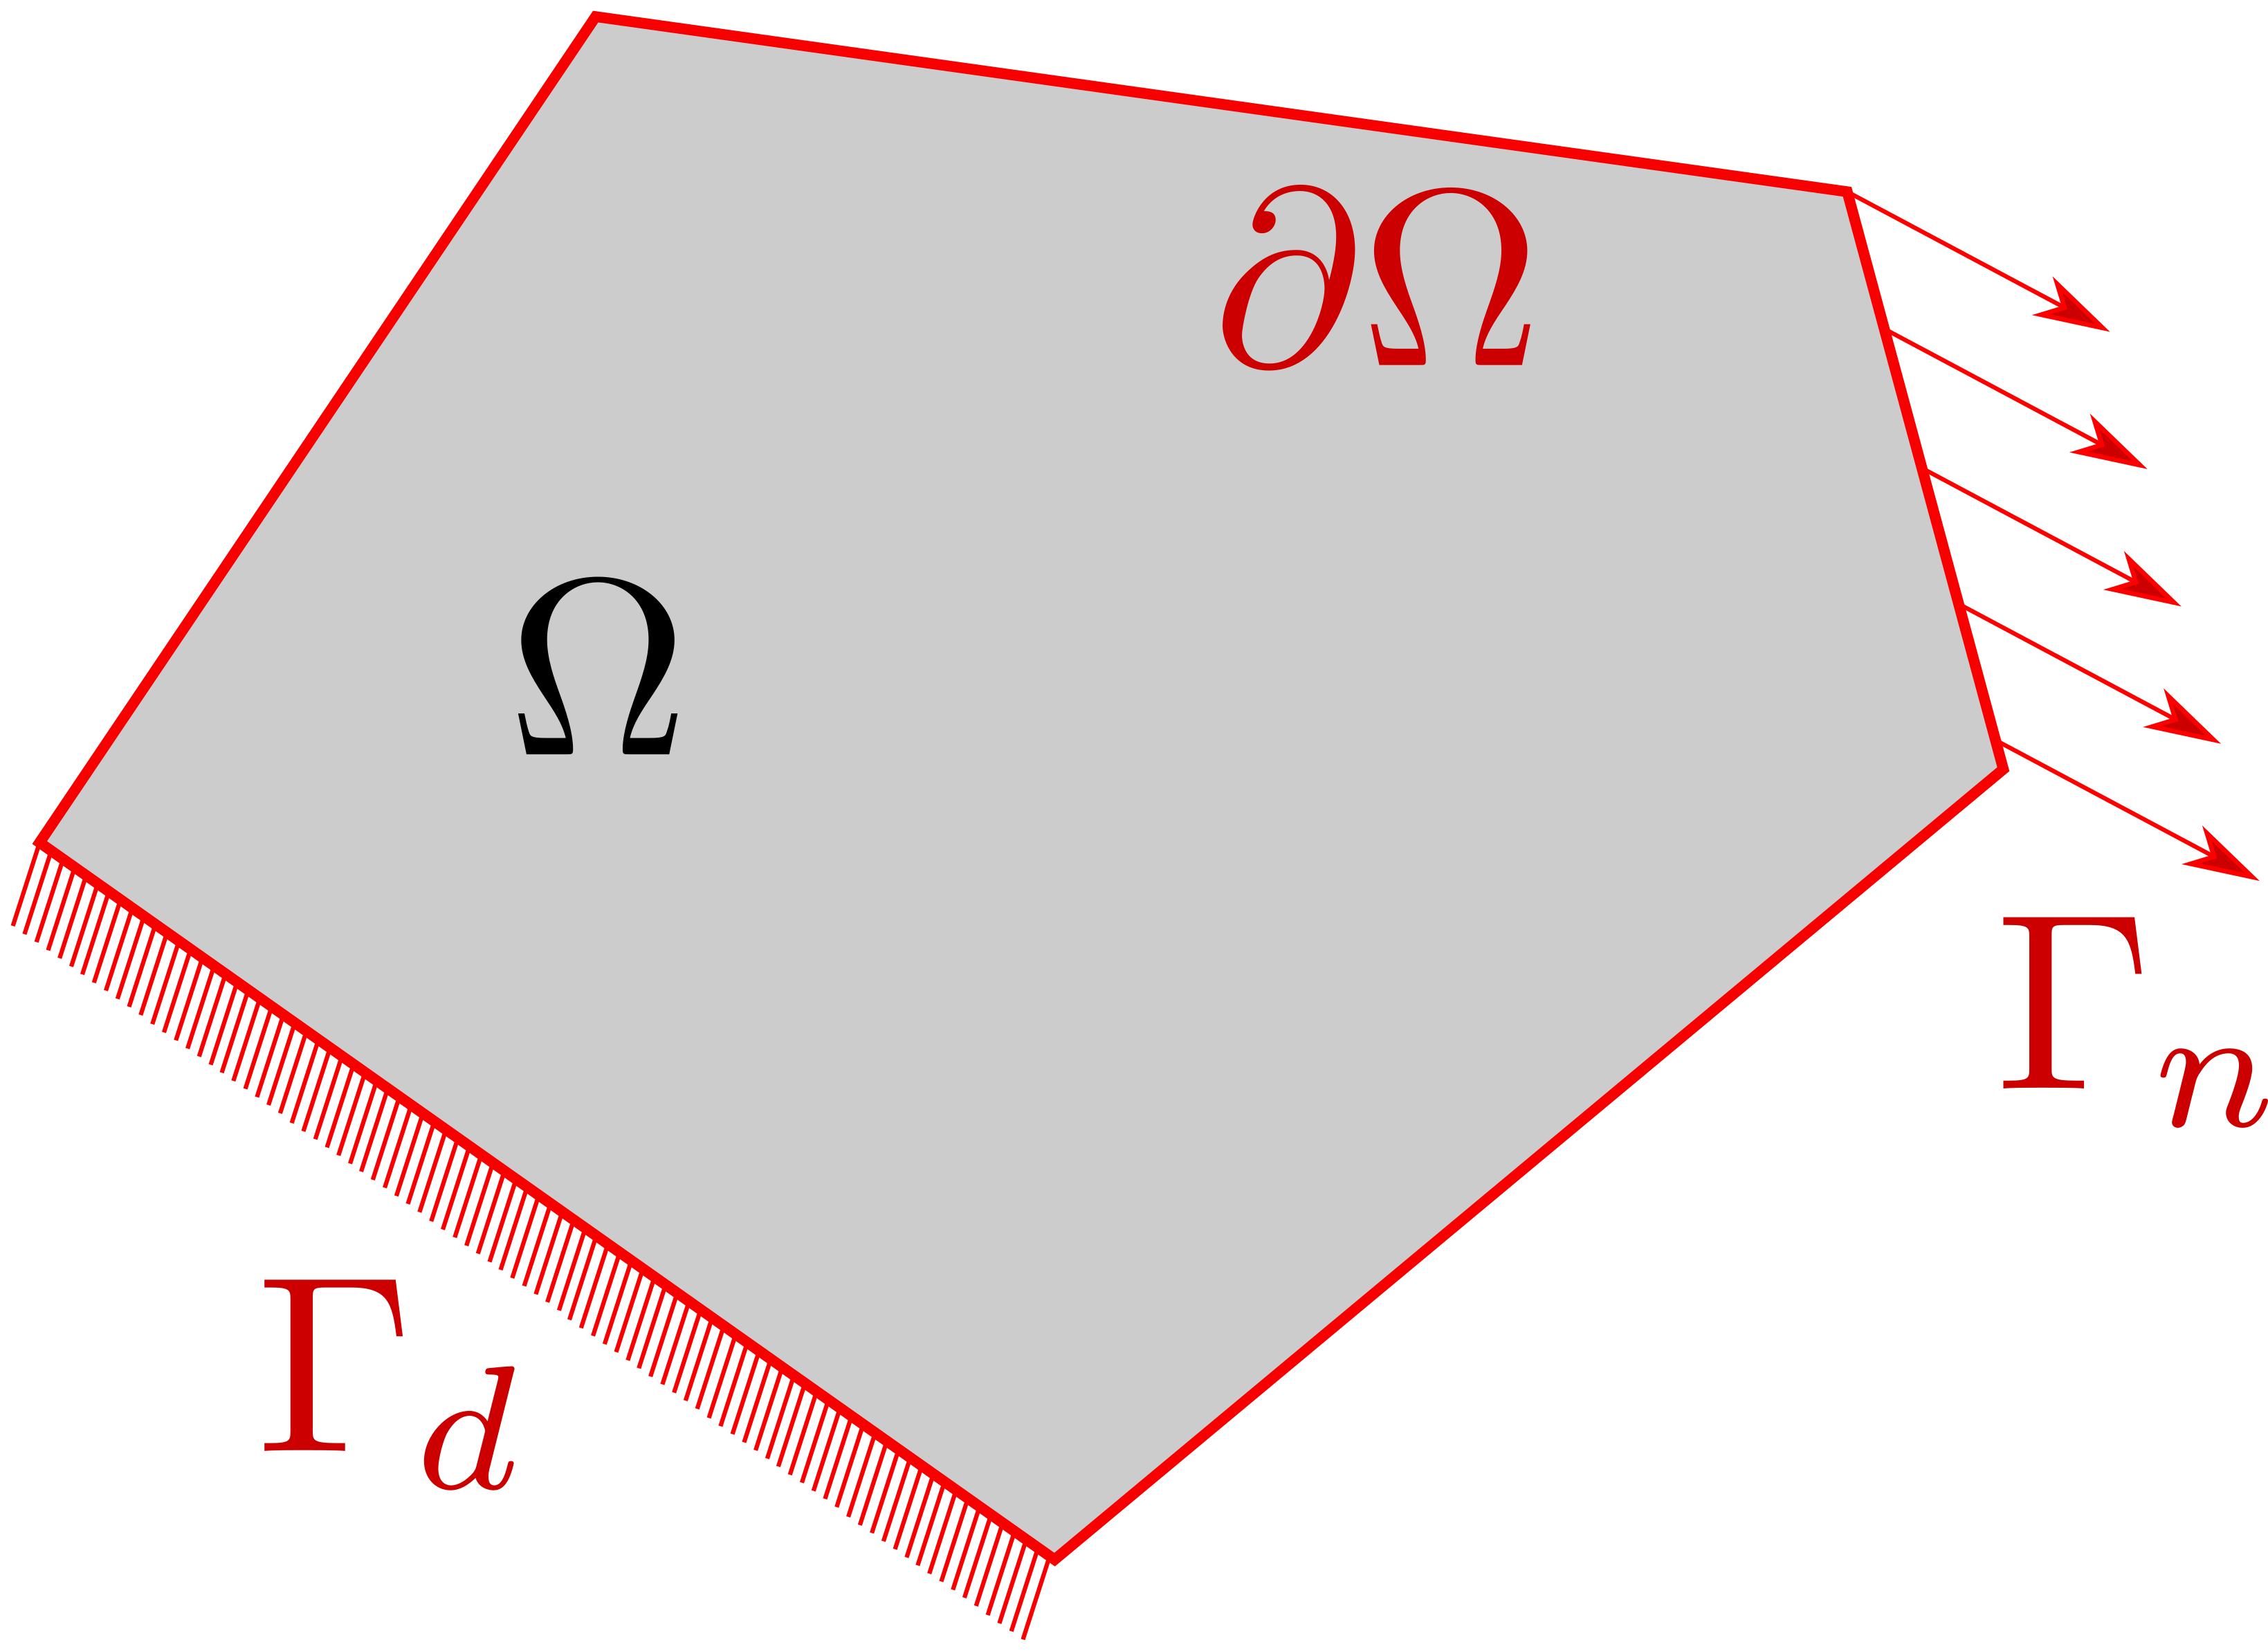
\includegraphics[width=\textwidth]{Figures/Continuum-solid}}
  \caption{Description of the boundary-value-problem in a
    continuum. Red lines represents the closure $\partial \varOmega$
    of the domain $\varOmega$ represented in gray.}
  \label{fig:Continuum-solid}
\end{figure}
%%%%%%%%%%%%%%%%%%%%%%%%%%%%%%%%%%%%%%%%%%%%%%%%%%%%%%%%%%%%%%%%%%%%%%%%%%
In this context the field \gls{u} allows to describe the \textit{global state}
of the system. Now the variable $\phi =
(\tens{\varepsilon},\tens{\sigma})$ is defined as the set of \textit{local
  states} at any point of the continuum which can be derived from the
field \gls{u} through the following set of governing equations and
restrictions that must be satisfied. \red{First (i) the \textit{compatibility
  equation}, where the the strain field \gls{strain} is extracted from \gls{u} is defined as:}
\begin{equation}
  \label{eq:Compatibility-equation}
  \tens{\varepsilon} = \GradS{\vect{u}},
\end{equation}
together with essential boundary conditions of Dirichlet type \gls{dirichlet-boundary}. An additional consideration over the strain field is
the assumption of inifinitesimal strain, therefore second order terms
in the spatial derivatives can be neglected. \red{Therefore, the stress field \gls{stress} will be considered the corresponding conjugate variable for the strain field, being the one} which satisfies (ii) the \textit{conservation of
  momentum equation}:
\begin{equation}
  \label{eq:Balance-momentum}
\rho \frac{D\vect{v}}{Dt} = \Div{\tens{\sigma}} + \rho \vect{b}
\end{equation}
together with the natural boundary conditions of the Neumann type \gls{neumann-boundary}.  An aditional component will be (iii) the constitutive equation as a linear
application from $\Re^n$ to $\Re^n$, which relates the
strain tensor with the stress tensor:
\begin{equation}
  \label{eq:Constitutive-equation}
\tens{\sigma} = \tens{D} \colon \tens{\varepsilon}.
\end{equation}
\red{In this research, plane strain Linear Elasticity has been considered. Thus the constitutive tensor, \tens{D}, is the well known linear elastic one.} The final restriction is (iv) the mass conservation, which can be obtained by
setting to zero the total derivative of the density field,
\begin{equation}
  \label{eq:Rho-material-derivative}
  \frac{D \rho}{D t} = \dot{\rho} + \rho \Div{\vect{v}} = 0.
\end{equation}

In order to obtain the variational statement of the problem, let us define a
virtual displacement field such that
\begin{equation}
  \label{eq:Hilbert-space}
  \vect{u}^{\psi} \in \mathcal{H}^1_0(\Omega) = \{ \vect{u}^{\psi} \in
  \mathcal{H}^1 \mid \vect{u}^{\psi} = \vect{0}\ \text{on}\ \Gamma_d \};
\end{equation}
satisfying that the Cauchy sequences are convergent in \gls{domain} as well:
\begin{equation}
  \label{eq:cauchy-secuence}
  \Integral{3}{\vect{u}^{\psi}} < \infty\ \quad\text{and}\quad
  \Integral{3}{\tens{\varepsilon}^{\psi}} < \infty.
\end{equation}
The principle of virtual work states that the equilibrium solution to
the boundary-value problem of elasticity is the function $\vect{u} \in
\mathcal{H}^1_0$ such that, for $\vect{u}^{\psi} \in
\mathcal{H}^1_0$, the following holds:
\begin{equation}
  \label{eq:BalanceMomentum_wf}
  \Integral{3}{\rho\ \left( \frac{d\vec{v}}{dt}\ - \vec{b} \right) \cdot \vec{u}^{\psi}} =
  \Integral{2}{\vec{t}\ \cdot \vec{u}^{\psi}} - \Integral{3}{\tens{\sigma} \colon
   \tens{\varepsilon}^{\psi}}.
\end{equation}\\
Thus, equation~\eqref{eq:BalanceMomentum_wf}, together with
\eqref{eq:Constitutive-equation} and
\eqref{eq:Rho-material-derivative}, represents the weak form
formulation of the problem.

In order to obtain a finite set of equations, in contrast with the
\acrshort{fem}, in \acrshort{mpm} a double discretization procedure is
performed. First, the continuum \gls{domain} is discretized with a finite sum of material points (also denominated particles the manuscript). Each material point
represents a part of the discretized domain $\varOmega_p \subset
\varOmega$ with $p = 1,2\ldots ,N_p$ where $N_p$ is the number of
particles. The material point location, $\vec{x}_p$, is defined at the centroid
of each $\Omega_p$ (see figure~\ref{fig:MPM-discretization} for details).
Initial values of position,
velocity, mass, volume and stress denoted by $\vec{x}_p$,
$\vec{v}_p$, $m_p$,  $V_p$ and $\tens{\sigma}_p$ respectively are assigned to each material point, which also owns the
virtual displacement field $\vect{u}^{\psi}_{p}$. Therefore, employing
the definition of the material integral, where Riemann \red{ALGUNA CITA AQUI}
integral definition is recovered as an addition of a finite set of points, and
their volumes are interpreted as quadrature weights. Consequently,
individual terms in \eqref{eq:BalanceMomentum_wf} are solved as follows. 
\begin{itemize}
\item Acceleration forces :
\begin{equation}
    \label{eq:particle_acceleration_forces}
    \Integral{3}{\rho\ \frac{d\vec{v}}{dt} \cdot \vect{u}^{\psi}} =
    \frac{d\vec{v}_{p}}{dt} \cdot \vect{u}^{\psi}_{p}\ m_p.
  \end{equation}\\
\item Internal forces :
  \begin{equation}
    \label{eq:particle_internal_forces}
    \Integral{3}{\tens{\sigma}\ \colon \tens{\varepsilon}^{\psi}} =
   \tens{\sigma}_{p}\ \colon \tens{\varepsilon}^{\psi}_p \ V_p.
  \end{equation}\\
\item Body forces :
\begin{equation}
  \label{eq:particle_body_forces}
  \Integral{3}{\rho\ \vec{b} \cdot \vect{u}^{\psi} } = 
  \vec{b}_{p} \cdot \vect{u}^{\psi}_p\ m_p.
\end{equation}\\
\item Loads :
\begin{equation}
  \begin{aligned}
    \label{eq:particle_load_forces}
    \Integral{2}{\vec{t}\ \vect{u}^{\psi}} = \Integral{2}{\rho\
      \vec{t}^s \cdot \vect{u}^{\psi}} = \vec{t}^s_{p} \cdot \vect{u}^{\psi}_{p}\ h^{-1}\ m_p ,
  \end{aligned} 
\end{equation}
\end{itemize}
where $h$ is the thickness of the continuum in a 2D case. Following, the aforementioned second discretization procedure appears. A background mesh
composed by a finite set of grid points with coordinates $\vec{x}_I\
, I = 1,2\ldots ,N_n$, is generated, being $N_n$ the number of grid
nodes. \red{Spatial derivatives, such as gradients and
divergences, are computed through the support of the background mesh.}

%%%%%%%%%%%%%%%%%%%%%%%%%%%%%%%%%%%%%%%%%%%%%%%%%%%%%%%%%%%%%%%%%%%%%%%%%%
\begin{figure}\sidecaption
  \centering
  \resizebox{0.5\hsize}{!}{
    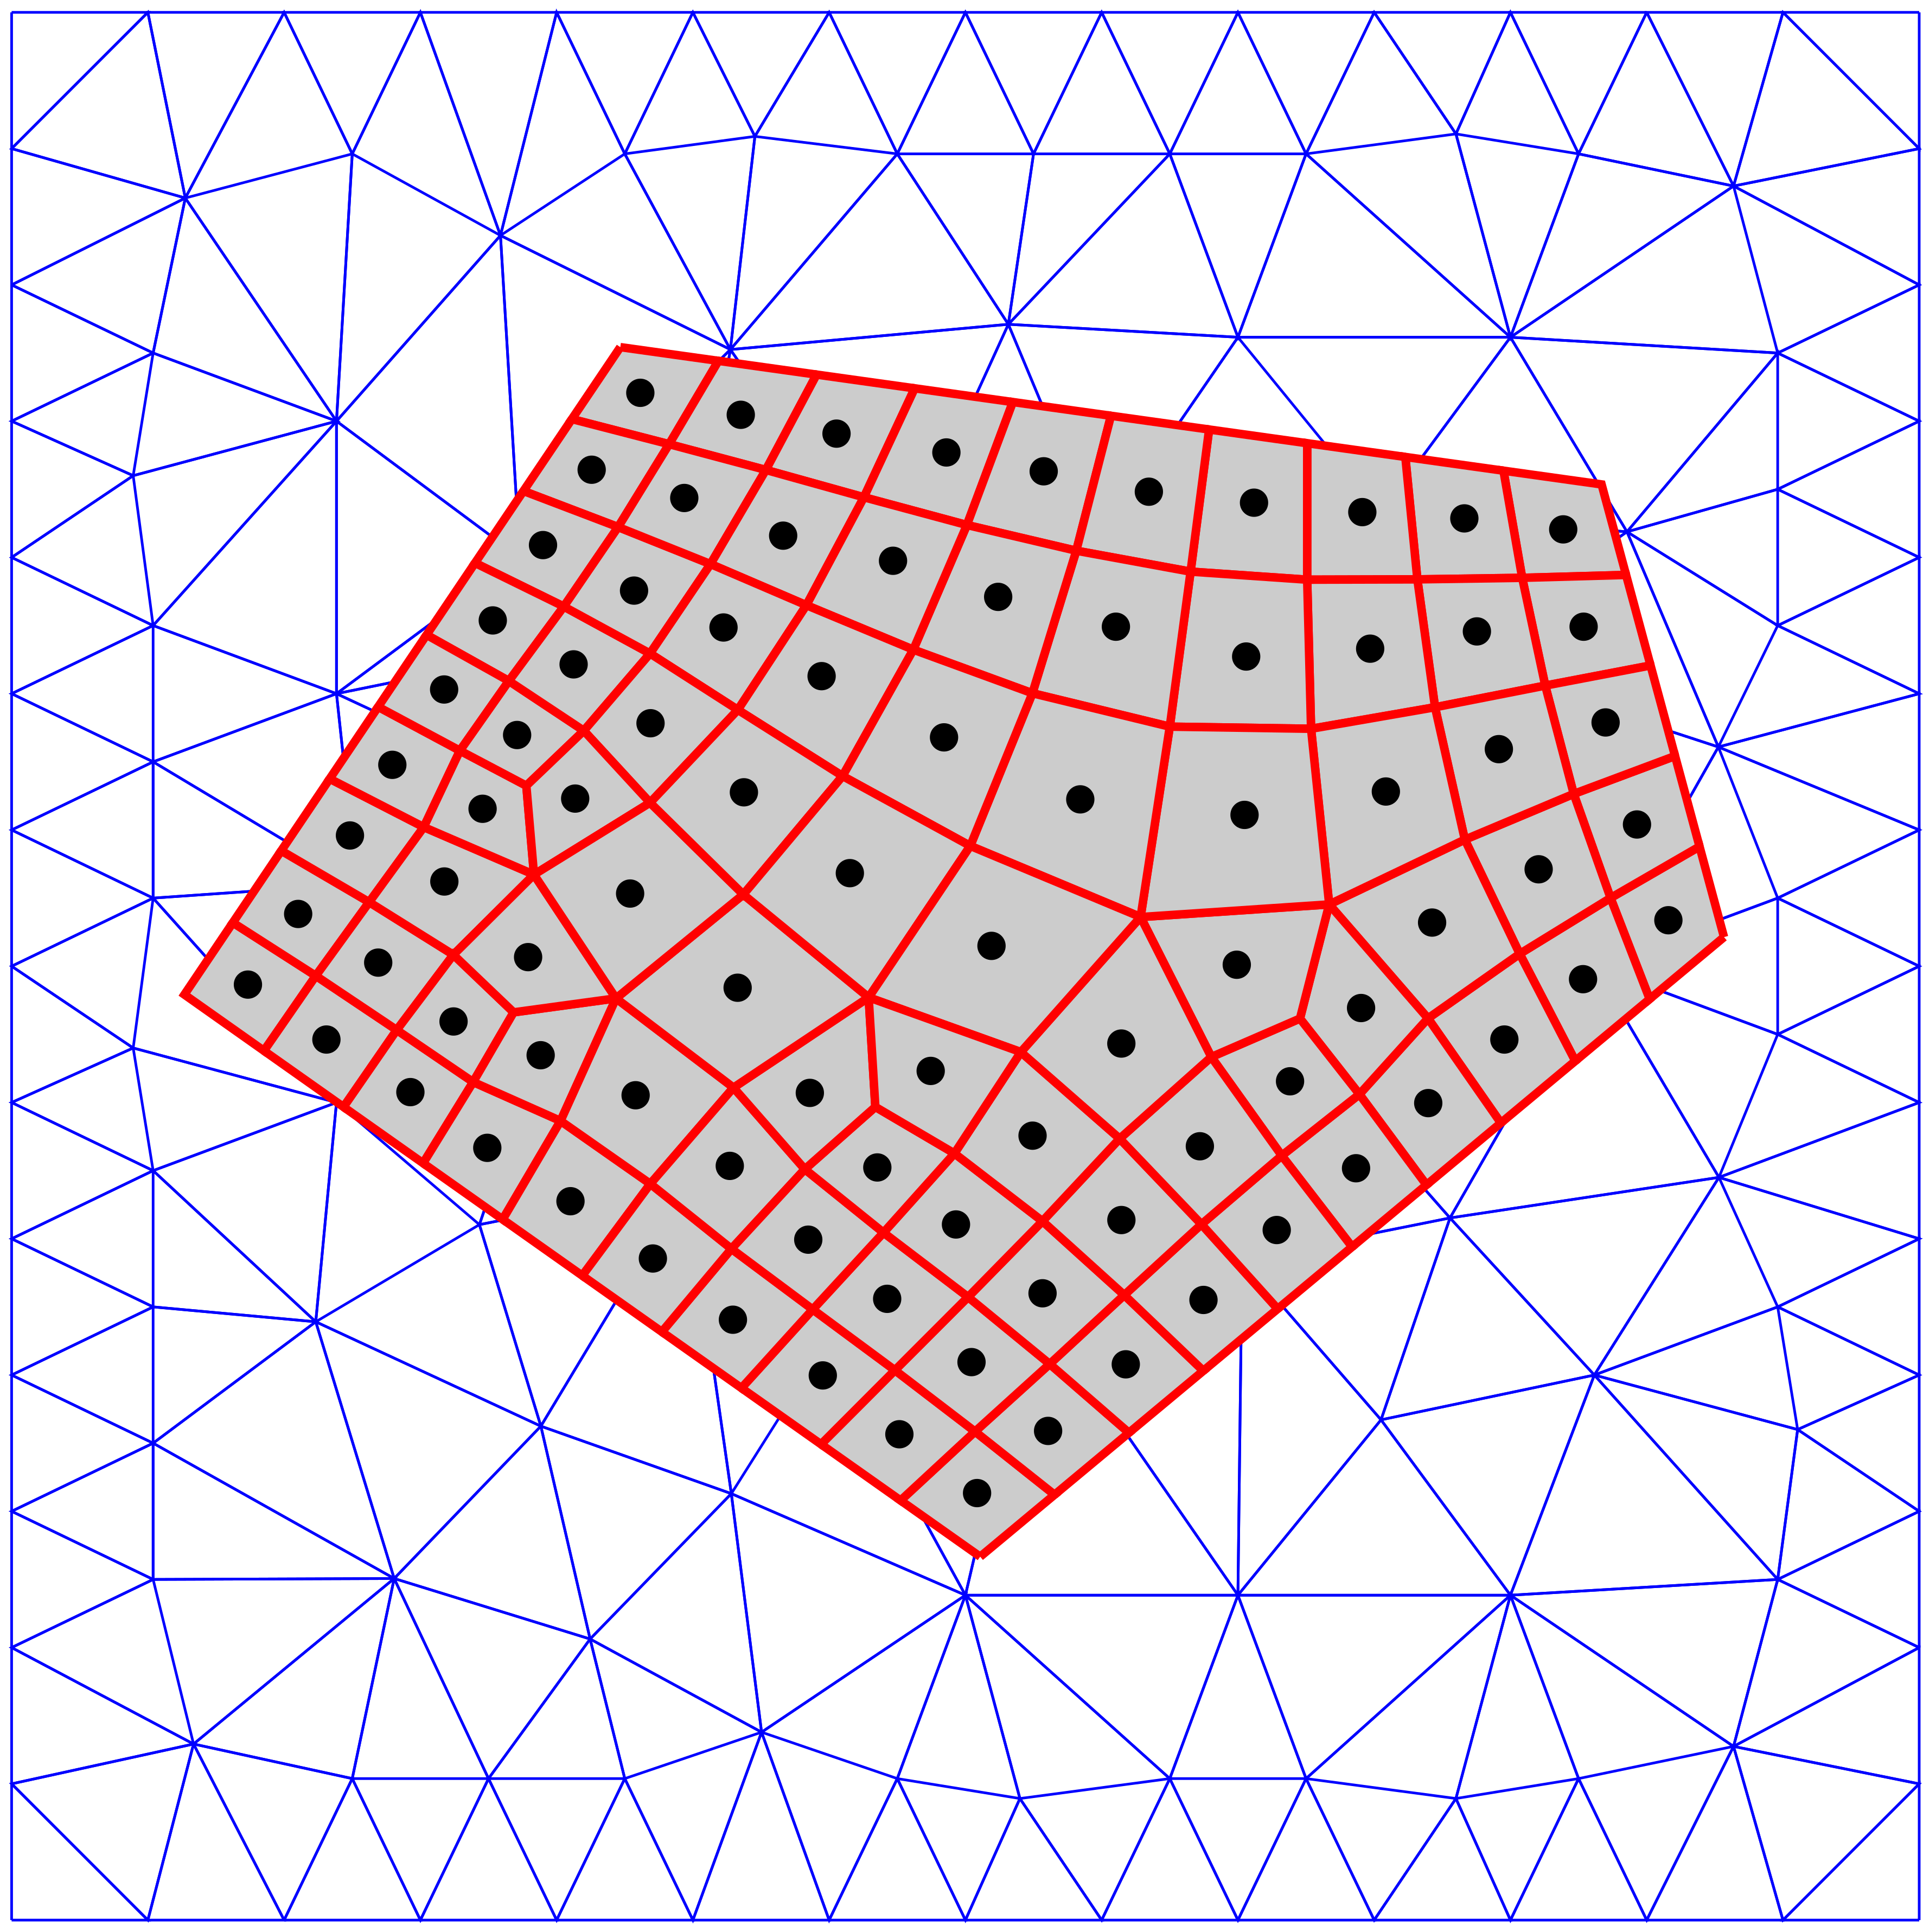
\includegraphics[width=\textwidth]{Figures/Mesh-particles-back}}
  \caption{Description of the spatial discretization for domain presented in the
    figure~\ref{fig:Continuum-solid}. Blue mesh represent the
    background computational support, and the red mesh conforms the
    discretized continuum body.}
  \label{fig:MPM-discretization}
\end{figure}
%%%%%%%%%%%%%%%%%%%%%%%%%%%%%%%%%%%%%%%%%%%%%%%%%%%%%%%%%%%%%%%%%%%%%%%%%%
Introducing \eqref{eq:particle_acceleration_forces},
\eqref{eq:particle_internal_forces}, \eqref{eq:particle_body_forces},  \eqref{eq:particle_load_forces} in \eqref{eq:BalanceMomentum_wf},
approximating the displacement field of the particle
$p$ as $\vec{u}_{p} = N_{Ip} \vect{u}_I$, $\vec{u}^{\psi}_{p} = N_{Ip} \vect{u}_I^{\psi}$,
and its gradient as $\tens{\varepsilon}_p = (\vect{u}_I \otimes
\Grad{N_{Ip}})^s$, $\tens{\varepsilon}_p^{\psi}= (\vect{u}_I^{\psi} \otimes \Grad{N_{Ip}})^s$.
nodal balance of forces of the continuum yields:
\begin{equation}
  \label{eq:particle_balance_forces3}
  \dot{\vec{p}}_{I}= \tens{m}_{IJ}\dot{\vec{v}}_{J} = \vec{f}_{I}^{int} + \vec{f}_{I}^{ext},
\end{equation}
where $\dot{\vec{p}}_{I}$ is the rate of momentum at grid node $I$ and $\tens{m}_{IJ}$, the nodal mass matrix, is obtained through:
\begin{equation}
  \label{eq:particle_nod_mass}
  \tens{m}_{IJ} = N_{Ip} m_p N_{Jp}.
\end{equation}
In order to improve the computational efficiency and stability, the nodal mass matrix
\eqref{eq:particle_nod_mass} can be substituted by the lumped mass
matrix $\tens{m}_{IJ}^{lumped}$.
Following, internal and external forces are computed as follows,
\begin{equation}
  \label{eq:nodal_internal_forces}
  \vec{f}_{I}^{int} = - \tens{\sigma}_{p} \cdot \Grad{N_{Ip}} \frac{m_p}{\rho_p}
\end{equation}
\begin{equation}
  \label{eq:nodal_external_forces}
  \vec{f}_{I}^{ext} = N_{Ip}\ \vec{b}_{p}\ m_p  + N_{Ip}\ \vec{t}^s_{p}\ m_p h^{-1} 
\end{equation}
where $\tens{\sigma}_{p} = \tens{\sigma}_{p}(\tens{\varepsilon}_{p})$
is the particle $p$ stress field, which can be integrated employing
the suitable constitutive model. The strain tensor rate, $\dot{ \tens{\varepsilon}}_{p}$, as a measure of the time derivative of the strain tensor, is updated employing the velocity at the background mesh by the equation:
\begin{equation}
  \label{eq:IncrStrainPoint}
  \dot{\tens{\varepsilon}_{p}} = \frac{\Delta
    \tens{\varepsilon}_{p}}{\Delta t} =
  \frac{1}{2} \left[\Grad{N_{Ip}}\ \otimes \vec{v}_{I} + \vec{v}_{I} \otimes
    \Grad{N_{Ip}}\ \right].
\end{equation}
Next, mass conservation is guaranteed by enforcing the null value of
the material derivative of the density field $\frac{D \rho}{D t} = 0$.
This leads to a suitable equation to update the density field:
\begin{equation}
  \label{eq:MassConservation}
\dot{\rho} = - \rho\ \mathit{trace} \left( \dot{\tens{\varepsilon}} \right).
\end{equation}
Finally, to solve the equation \eqref{eq:particle_balance_forces3}, a second order
\cancel{temporal} \red{time} integration scheme is required. Therefore, time is
discretized into a finite set of time steps $k = 1\ldots ,Nt$, where $k$ is the current time step and $N_t$
is the total number of time steps. Once the nodal equilibrium equation is solved, the values at the nodes are
interpolated back into the particles, which are advected
to the new position through:
\begin{equation}
  \label{eq:Updated_Lagrangian}
  \dot{\vec{v}}_p = N_{Ip}\ \vec{a}_{I},\quad and\quad
  \dot{\vec{x}}_{p} = N_{Ip}\ \vec{v}_{I}  
\end{equation}
\red{Traditionally, Eqs.
\eqref{eq:particle_balance_forces3} and ~\eqref{eq:Updated_Lagrangian},
are solved with an explicit forward Euler algorithm. In the following subsection, this and the proposed schemes are described}.


\subsection{\acrshort{mpm} time integration scheme: the Explicit Predictor-Corrector proposal}
%\subsection{Explicit predictor-corrector scheme for \acrshort{mpm}.}
\label{sec:epc-algor-mpm}

\red{As was stated previosuly, an explicit forward Euler algorithm has been utilized widely within the \acrshort{MPM} methodology. This scheme has been described in detail by many researchers
\cite{Sulsky1994}, \cite{Bardenhagen2002}, \cite{thesis_Andersen_2009} and can be sketched by the scheme of the figure~\ref{fig:MPM_algorithm}.}
%%%%%%%%%%%%%%%%%%%%%%%%%%%%%%%%%%%%%%%%%%%%%%%%%%%%%%%%%%%%%%%%%%%%%%%%%%
\begin{figure}\sidecaption
  \centering
  \resizebox{0.8\hsize}{!}{
    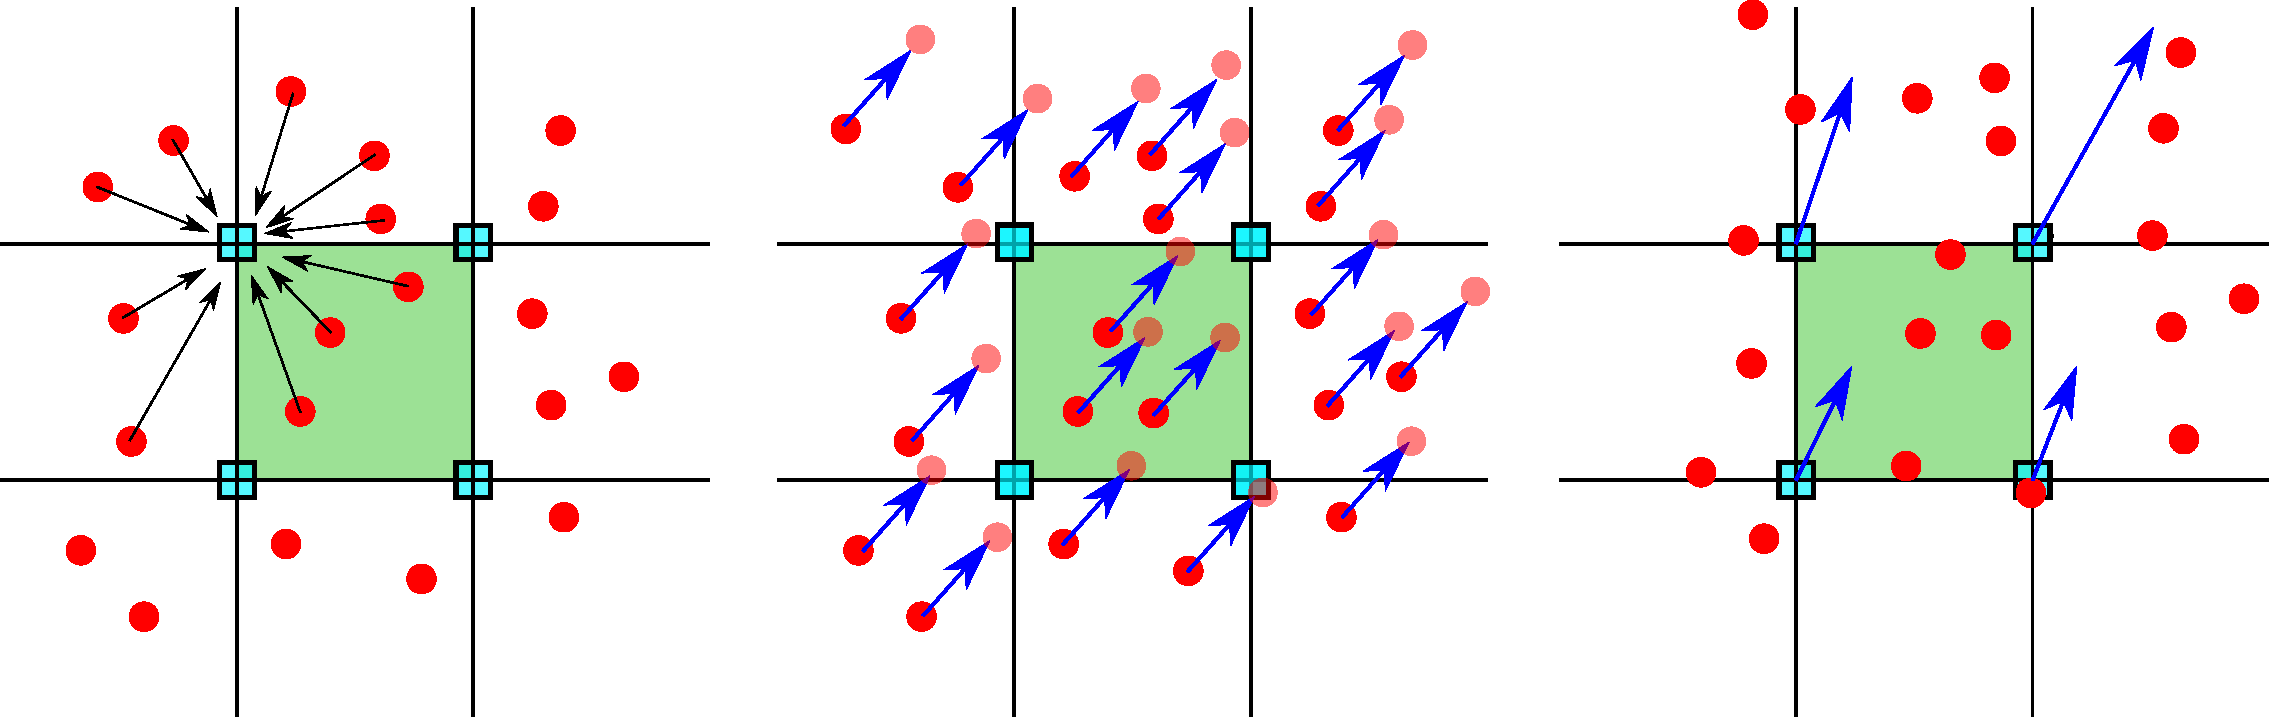
\includegraphics[width=\textwidth]{./Figures/MPM_scheme_horizontal}
  }
  \caption{Description of the three steps in \acrshort{mpm} standard algorithm.}
  \label{fig:MPM_algorithm}
\end{figure}
%%%%%%%%%%%%%%%%%%%%%%%%%%%%%%%%%%%%%%%%%%%%%%%%%%%%%%%%%%%%%%%%%%%%%%%%%%
Other authors have proposed many others time integration alternatives
like \cite{Guilkey2003}, \cite{Tran2019e}, \cite{Charlton2017}. In the
first publication on \acrshort{mpm} \cite{Sulsky1994}, the nodal acceleration
was employed to update the particles as
\begin{equation}
  \label{eq:Sulsky-1994-UL-v}
  \vect{v}_p^{k+1} = \vect{v}_p^{k} + \Delta t\ N_{Ip}^{k}\ \vec{a}_{I}^{k}
\end{equation}
\begin{equation}
  \label{eq:Sulsky-1994-UL-x}
  \vect{x}_p^{k+1} = \vect{x}_p^{k} + \Delta t\ N_{Ip}^{k}\ \vec{v}_{I}^{k}.
\end{equation}
However, as Andersen (2009)\cite{thesis_Andersen_2009} pointed out, this algorithm has been shown to be numerically unstable due to that
$\vect{f}_I^{int,k}$ can be finite for an infinitesimal nodal mass
$\tens{m}$\red{NO ENTIENDO??}. This issue may lead to numerical issues when nodal acceleration
is obtained in the evaluation of the Eqs. \eqref{eq:Sulsky-1994-UL-x} and \eqref{eq:Sulsky-1994-UL-v}. Hence, a
corrected version of this algorithm was proposed by Zhang {\it et al.}
(2016)\cite{Zhang_book_2016}:
\begin{equation}
  \label{eq:Zhang-2016-UL-x}
  \vect{x}_p^{k+1} = \vect{x}_p^{k} + \Delta t\ \frac{N_{Ip}^{k}\ \vec{p}_{I}^{k}}{\tens{m}_I}, 
\end{equation}
\begin{equation}
  \label{eq:Zhang-2016-UL-v}
  \vect{v}_p^{k+1} = \vect{v}_p^{k} + \Delta t\ \frac{N_{Ip}^{k}\ \vec{f}_{I}^{k}}{\tens{m}_I}.
\end{equation}
Delving into the improvement of the accuracy of the \acrshort{mpm} explicit schemes, Tran \& Solowski (2019)\cite{Tran2019e} presented a
generalized-$\alpha$ scheme for \acrshort{mpm} inspired in the explicit time
integration algorithm proposed by Chung \& Hulbert
(1993)\cite{Geranlized_alpha_1993}, but with the particularity that
the acceleration is evaluated both in the beginning and the end of the
time step.
\begin{equation}
  \label{eq:Tran-2019-GA-v}
  \vect{v}_p^{k+1} = \vect{v}_p^{k} + \Delta t\  N_{Ip}^{k}\ \left[(1 - \gamma)\ \vect{a}_I^{k} +
    \gamma\ \vect{a}_I^{k+1} \right],\\
\end{equation}
\begin{equation}
\label{eq:Tran-2019-GA-x}
  \vect{x}_p^{k+1} = \vect{x}_p^{k} + N_{Ip}^{k} \left[ \Delta t\ \vec{v}_{I}^{k}+ \Delta t^2\left( (\frac{1}{2} - \beta)\
    \vec{a}_{I}^{k} + \beta\ \vec{a}_{I}^{k+1} \right) \right],
\end{equation}
\begin{equation}
  \label{eq:Tran-2019-GA-a}
  \vect{a}_p^{k+1} = N_{Ip}^{k}\ \vec{a}_{I}^{k+1}.
\end{equation}

This scheme has been proven to damps out the highest frequency noises
\cite{Tran2019e}. However, it can present the same numerical instabilities
as in \eqref{eq:Sulsky-1994-UL-x},\eqref{eq:Sulsky-1994-UL-v} when
nodal masses become infinitesimal, and requires extra storage for
nodal values of acceleration and previous steps.

In this section, an explicit predictor-corrector time integration
scheme is proposed. It is based on the Newmark central differences explicit scheme, which is also denominated a-form 
$\gamma = 0.5$ and $\beta = 0$. This method is devoted to solve a system of equations of the type
\begin{equation*}
  \Matrix{M}_{IJ}\ddot{\Vector{d}}_{J} + \Matrix{C}_{IJ}\dot{\Vector{d}}_{J} +
  \Matrix{K}_{IJ}\Vector{d}_{J} = \Vector{F}_{I}.
\end{equation*}
\red{The nodal \acrshort{mpm} stage allows to apply this method
in the \acrshort{mpm} framework in a similar manner that the one
proposed by Tran~\it{et al.}~\cite{Tran2019e}. Taking into account the predictor definition, it is possible to calculate
nodal velocities and update particles position employing nodal values
of velocity and acceleration.} 

The predictor-corrector algorithm has
been described in the classic literature \cite{Hughes2000}, and its
stability and computational advantages were widely proven by Liu
\cite{Xiaojian94}. The ``classic'' \acrfull{npc} algorithm starts with a
predicted value of the nodal velocities at the $(k+1)$th time step, denoted by $\vec{\tilde{v}}_I^{k+1}$, which is calculated as follows:
\begin{equation}
  \label{eq:Predictor-velocity-I}
  \vec{\tilde{v}}_I^{k+1} = \vec{v}_I^k + (1 - \gamma)\ \Delta t\ \vec{a}_I^k.
\end{equation}

The \textit{user-defined}
parameter $\gamma \geq 0$ that appears in In \eqref{eq:Predictor-velocity-I}, influences both the predictor accuracy
and the stability of the algorithm. As pointed out Liu
\cite{Xiaojian94}, the truncation error of the predictor formula is
$O(\Delta t^3)$ when $\gamma = 0.5$, and is unconditionally stable if
$ 0 < \gamma \leq 0.25$.

To accommodate this step to \acrshort{mpm} framework, it is necessary to get
the nodal values of the velocity and acceleration throughout a variational
recovery process where particles quantities are transferred to the
mesh nodes. This technique arises as a generalization of the super-convergent recovery
procedures described by Zienkiewicz \& Zhu \cite{ZZ1992_I} (\textit{ZZ})
in the context of \acrshort{fem}. In \acrshort{mpm}, Gauss quadratures are not employed. However, 
integrals are computed following the Riemann integral definition,
where each component of the summation corresponds to a particle of the
discretization. Also Bardenhagen \& Kober \cite{Bardenhagen2004}
proved that through this information-transference technique mass and momentum are conserved. So for a general particle variable $\Phi_p$, employing the
\textit{ZZ} technique, it is possible to get its nodal homologous $\Phi_I$  as:
\begin{equation}
  \label{eq:Variational-recovery}
   \Phi_I = \frac{m_p N_{Ip} \Phi_p}{m_I}.
 \end{equation}
 Therefore, to get an analogous expression for
 \eqref{eq:Predictor-velocity-I} in the context of \acrshort{mpm}, the
 procedure described in the equation \eqref{eq:Variational-recovery}
 is employed, obtainen the following expression:
 \begin{equation}
   \label{eq:Predictor-velocity-II}
   \vec{\tilde{v}}_I^{k+1} = \underbrace{\frac{N_{Ip}^{k} m_p
       \vec{v}_p^k}{m_I}}_{\vec{v}_I^{k}} + (1 - \gamma)\ \Delta t\  \underbrace{\frac{N_{Ip}^{k} m_p \vec{a}_p^k}{m_I}}_{\vec{a}_I^{k}}.
 \end{equation}
Nonetheless this way of computing the predictor stage can introduce
instabilities due to numerical cancellation likewise the original
Sulky algorithm. Thankfully, this can be avoided easily by the
equivalent formulation proposed as follows: 
\begin{equation}
  \label{eq:Predictor-velocity-II}
  \vec{\tilde{v}}_I^{k+1} = \frac{ N_{Ip}^{k} m_p (\vec{v}_p^k + (1 - \gamma)\ \Delta t\ \vec{a}_p^k)}{m_I}.
\end{equation}
This way of computing the nodal predictor is both numerically stable
and minimize the computational effort. Once nodal velocities are
obtained, the essential boundary conditions are imposed over \gls{dirichlet-boundary}. And in the
following, the ``classic'' \acrshort{mpm} algorithm continues to reach to the
equilibrium equation \eqref{eq:particle_balance_forces3}. Next, the
\textit{corrector} stage is introduced. Due to the fact that nodal
velocities were obtained earlier, this step is computed in the same way as
in \acrshort{fem},
\begin{equation}
  \label{eq:Corrector-velocity}
  \vec{v}_{I}^{k+1} = \vec{v}_{I}^{pred} + \gamma\ \Delta t\ \frac{\vec{f}_{I}^{k+1}}{\tens{m}_I^{k+1}}.
\end{equation}
Finally updated particle kinetics are computed using nodal values as:
\begin{align}
  \label{eq:Update-lagrangian-pce}
        &\vec{a}_p^{k+1} = \frac{N_{Ip}^k\vec{f}_{I}^{k}}{\tens{m}_I^k}\\
      &\vec{v}_p^{k+1} = \vec{v}_p^n + \Delta t\
        \frac{N_{Ip}^k\
        \vec{f}_{I}^{k}}{\tens{m}_I^k}\\
      &\vec{x}_p^{k+1} = \vec{x}_p^n + \Delta t\
         N_{Ip}^k\ \vec{v}_{I}^{k} +
        \frac{1}{2}\Delta t^2\ \frac{N_{Ip}^k\
        \vec{f}_{I}^{k}}{\tens{m}_I^k}.
\end{align}
Notice that particle displacements are computed using the corrected
nodal velocities as well as the accelerations with the velocities
of the predictor. However, particle velocities and accelerations
are computed using the corrected velocities. Therefore here we share similarities
with the \textit{leapfrog integration} where position is not updated at
full time step, but the velocity is updated at half time steps. Notice
also that, with this approach, the calculation of nodal momentum values
are not required. Due to its simplicity, the proposed scheme can be implemented with minor modifications
over the standard forward Euler. The full implementation is summarized in the algorithm~\ref{algo:1}.

\begin{algorithm}
  \floatname{algorithm}{Algorithm 1}
  \renewcommand{\thealgorithm}{}
  \caption{\acrfull{npc} scheme} \label{algo:1}
  \begin{algorithmic}[1]
    %%%%%%%%%%%%%%%%%%%%%%%%%%%%%%%%%%%%%%%%%%%%%%%%%%%%%%%%%%%%%%%%%%%%%%%%%%%%%%%%%%%%%% º
    \STATE \textbf{Update mass matrix}:
    \begin{equation*}
      \tens{m}_{I} = N_{Ip}^{k}\ m_p,
    \end{equation*}
    %%%%%%%%%%%%%%%%%%%%%%%%%%%%%%%%%%%%%%%%%%%%%%%%%%%%%%%%%%%%%%%%%%%%%%%%%%%%%%%%%%%%%% 
    \STATE \textbf{Explicit Newmark Predictor}:\\
    \begin{equation*}
      \vec{v}_I^{pred} = \frac{ N_{Ip}^{k} m_p (\vec{v}_p^k + (1 - \gamma)\ \Delta t\ \vec{a}_p^k)}{m_I}
    \end{equation*}
    %%%%%%%%%%%%%%%%%%%%%%%%%%%%%%%%%%%%%%%%%%%%%%%%%%%%%%%%%%%%%%%%%%%%%%%%%%%%%%%%%%%%%% 
    \STATE \textbf{Impose essential boundary conditions}:\\
    At the fixed boundary, set $\vec{v}_{I}^{pred} = 0$. 
    %%%%%%%%%%%%%%%%%%%%%%%%%%%%%%%%%%%%%%%%%%%%%%%%%%%%%%%%%%%%%%%%%%%%%%%%%%%%%%%%%%%%%% 
    % \STATE \textbf{Discard the previous nodal values}.
    %%%%%%%%%%%%%%%%%%%%%%%%%%%%%%%%%%%%%%%%%%%%%%%%%%%%%%%%%%%%%%%%%%%%%%%%%%%%%%%%%%%%%% 
    \STATE \textbf{Deformation tensor increment calculation}.
    \begin{align*}
      &\dot{\tens{\varepsilon}_{p}}^{k+1} = \left[ \vec{v}_{I}^{pred} \otimes
        \Grad{N_{Ip}^{k+1}} \right]^s \\
      &\Delta \tens{\varepsilon}_{p}^{k+1} = \Delta t\ \dot{\tens{\varepsilon}_{p}}^{k+1}
    \end{align*}
    %%%%%%%%%%%%%%%%%%%%%%%%%%%%%%%%%%%%%%%%%%%%%%%%%%%%%%%%%%%%%%%%%%%%%%%%%%%%%%%%%%%%%% 
    \STATE \textbf{Update the density field}:
    \begin{equation*}
      \rho_p^{k+1} = \frac{\rho_p^k}{1 + \mathit{trace}\left[\Delta\tens{\varepsilon}_{p}^{k+1}\right]}.
    \end{equation*}
    %%%%%%%%%%%%%%%%%%%%%%%%%%%%%%%%%%%%%%%%%%%%%%%%%%%%%%%%%%%%%%%%%%%%%%%%%%%%%%%%%%%%%% 
    \STATE \textbf{Balance of forces calculation}:\\
    Calculate the total grid nodal force $\vec{f}_{I}^{k+1} =
    \vec{f}_{I}^{int,k+1} + \vec{f}_{I}^{ext,k+1}$ by evaluating
    \eqref{eq:nodal_internal_forces} and
    \eqref{eq:nodal_external_forces} in the time step $k+1$.
    In the grid node, $I$ is fixed in one of the spatial dimensions, set it to
    zero to make the grid nodal acceleration zero in that direction.\red{NO ENTIEND??}\\
    %%%%%%%%%%%%%%%%%%%%%%%%%%%%%%%%%%%%%%%%%%%%%%%%%%%%%%%%%%%%%%%%%%%%%%%%%%%%%%%%%%%%%% 
    \STATE \textbf{Explicit Newmark Corrector}:
    \begin{equation*}
      \vec{v}_{I}^{k+1} = \vec{v}_{I}^{pred} + \gamma\ \Delta t\ \frac{\vec{f}_{I}^{k+1}}{\tens{m}_I^{k+1}}  
    \end{equation*}
    %%%%%%%%%%%%%%%%%%%%%%%%%%%%%%%%%%%%%%%%%%%%%%%%%%%%%%%%%%%%%%%%%%%%%%%%%%%%%%%%%%%%%%
    \STATE \textbf{Update particles lagrangian quantities}:
    \begin{align*}
      &\vec{a}_p^{k+1} = \frac{N_{Ip}^k\vec{f}_{I}^{k}}{\tens{m}_I^k}\\
      &\vec{v}_p^{k+1} = \vec{v}_p^n + \Delta t\
        \frac{N_{Ip}^k\
        \vec{f}_{I}^{k}}{\tens{m}_I^k}\\
      &\vec{x}_p^{k+1} = \vec{x}_p^n + \Delta t\
         N_{Ip}^k\ \vec{v}_{I}^{k} +
        \frac{1}{2}\Delta t^2\ \frac{N_{Ip}^k\
        \vec{f}_{I}^{k}}{\tens{m}_I^k}
    \end{align*}
    %%%%%%%%%%%%%%%%%%%%%%%%%%%%%%%%%%%%%%%%%%%%%%%%%%%%%%%%%%%%%%%%%%%%%%%%%%%%%%%%%%%%%% 
    \STATE \textbf{Reset nodal values}
  \end{algorithmic}
\end{algorithm}

\subsection{Local \textit{max-ent} approximants}
\label{sec:local-max-ent}
The popularity of \acrshort{mpm} has increase notoriously during
the recent years due to its ability to deal with large strain problems
without mesh distorsion issues inherent to mesh based methods like
\acrshort{fem}, see Zdzislaw \cite{Wieckowski2004}. However, in the simulations
made with the original \acrshort{mpm}, there are numerical noises when particles
crossing the cell boundaries. \acrfull{lme} approximation schemes were
first introduced by Arroyo \& Ortiz (2006)\cite{Arroyo2006} has been
recently tested under \acrshort{mpm} framework by Wobbes {\it et al.}
(2020)\cite{Wobbes2020} where they prof that simulations performed
with \acrshort{lme}, shows considerably more accurate stress
approximations for \acrshort{mpm}. Although, in \cite{Wobbes2020}
authors does not deep in how the regularization parameter $\beta$
affects to the accuracy and stability of the solution. The basic idea
of the shape functions based on such an estimate is to interpret the shape function $N_I(\vec{x})$ as a probability. This allow us to introduce two important limits:
the principle of maximum-entropy (\textit{max-ent}) statistical
inference stated by \cite{Jaynes1957}, and the Delaunay triangulation
which ensures the minimal width of the shape function. 

This approximation scheme represents a optimal compromise, in the sense of
Pareto, between the \textit{unbiased statistical inference} based on
the nodal data which leads to the principle of \textit{maximum-entropy}
stated by Jaynes \cite{Jaynes1957}, and the definition of local shape
functions of \textit{least width} the least biased shape functions.

Taking the definition of entropy as a measure of how uncertainty a
random variable is averaged on all its possible outcomes. And adopting
the Shannon's entropy as the starting point:
\begin{equation}
  \label{eq:Shannon-entropy}
  H(p_1(\vec{x}),\ldots,p_n(\vec{x})) = -\sum^{N_n}_{I=1}{p_I(\vec{x})\log p_I }
\end{equation}
where $p_I(\vec{x})$ is the probability, equivalent to the mentioned
shape function $N_I(\vec{x})$, satisfying both the zeroth and
first-order consistency. The least-biased approximation scheme is
given by
\begin{align*}
  \label{eq:least-biased-approximation-scheme}
  \text{(LME)} \hspace{0.15cm} &\text{Maximize} \hspace{0.15cm} H(N_I) \equiv
  -\sum_{I}^{N_n}{N_I(\vec{x})\log N_I }\\
  &\text{subject to}\
  \begin{cases}
    N_I \ge 0, \hspace{0.15cm} \text{I=1, ..., n} \\[1em]   
    \sum\limits_{I=1}^{N_n}{N_I} = 1 \\[1em]   
    \sum\limits_{I=1}^{N_n}{N_I \vec{x}_I} = \vec{x} \\
  \end{cases}
\end{align*}
On the other hand, the control of the shape function width and its
dacay with distance away from the corresponding nodes is a desirable property. To reach to this objective \cite{Arroyo2006} propose the following linear program,
\begin{align*}
  \label{eq:RAJAN}
  \text{(RAJ)} \hspace{0.15cm} &\text{For fixed} \hspace{0.15cm}
  \vec{x} \hspace{0.15cm} \text{minimize} \hspace{0.15cm} U(\vec{x}_p,N_I) \equiv
\sum_I N_I |\vec{x}_p - \vec{x}_I |^2\\
  &\text{subject to}\
  \begin{cases}
    N_I \ge 0, \hspace{0.15cm} \text{I=1, ..., n} \\[1em]   
    \sum\limits_{I=1}^{N_n}{N_I} = 1 \\[1em]   
    \sum\limits_{I=1}^{N_n}{N_I \vec{x}_I} = \vec{x} \\
  \end{cases}
\end{align*}
To reach to a compromise between two competing objectives, a Pareto set is defined by \cite{Arroyo2006} as,
\begin{align*}
  \label{eq:LME-scheme-pareto-set}
  \text{(LME)}_{\beta} \hspace{0.15cm} &\text{For fixed} \hspace{0.15cm}
  \vec{x} \hspace{0.15cm} \text{minimize} \hspace{0.15cm} f_{\beta}(\vec{x}, N_I) \equiv \beta U(\vec{x},N_I) - H(N_I) \\
  &\text{subject to}\
  \begin{cases}
    N_I \ge 0, \hspace{0.15cm} \text{I=1, ..., n} \\[1em]   
    \sum\limits_{I=1}^{N_n}{N_I} = 1 \\[1em]   
    \sum\limits_{I=1}^{N_n}{N_I \vec{x}_I} = \vec{x} \\
  \end{cases}
\end{align*}
The regularization o \textit{thermalization} parameter
between the two criterion $\beta$ has Pareto optimal values in the range
$\beta \in (0,\infty)$. The unique solution of
the local \textit{max-ent} problem \acrshort{lme}$_\beta$ is:
\begin{equation}
  \label{eq:LME-p}
N_I^*(\vec{x})=\frac{\exp\left[ -\beta \; |\vec{x}-\vec{x}_I|^2 +
    \vec{\lambda}^* \cdot (\vec{x}-\vec{x}_I) \right] } {Z(\vec{x},\vec{\lambda}^*)}
\end{equation}
where
\begin{equation}
  \label{eq:LME-Z}
Z(\vec{x}, {\vec{\lambda}}) = \sum_{I=1}^{N_n}{ \exp \left[ -\beta \; |\vec{x}-\vec{x}_I|^2 + \vec{\lambda} \cdot (\vec{x}-\vec{x}_I)  \right]}
\end{equation}
being $\vec{\lambda}^*(\vec{x})$ the unique minimiser for the function $\log
Z(\vec{x}, \vec{\lambda})$. The traditional way to obtain such a minimiser is using Eq.~(\ref{eq:LME-J}) to calculate small increments of $\partial\vec{\lambda}$ in a Newton-Raphson approach. Where $\tens{J}$ is the Hessian matrix, defined by:
\begin{eqnarray}
  \label{eq:LME-J} 
  \tens{J}(\vec{x}, \vec{\lambda},\beta) &\equiv& \frac{\partial
                                                  \vec{r}}{\partial \vec{\lambda}}\\
  \label{eq:LME-r}
  \vec{r}(\vec{x},\vec{\lambda},\beta) &\equiv& \frac{\partial \log{ Z(   \vec{x},\vec{\lambda}})}{\partial \vec{\lambda}}  = \sum_I^{N_n} p_I(\vec{x},\vec{\lambda},\beta) \, (\vec{x} - \vec{x}_I)
\end{eqnarray}
In order to obtain the first derivatives of the shape function, it is also necessary to compute~$\nabla N_I^*$
\begin{equation}
  \label{eq:LME-grad-p}
\nabla N_I^* &=& N^*_I  \, \left(\nabla f^*_I-\sum_J^{N_n} N^*_J \, \nabla f^*_J\right)
\end{equation}
where
\begin{equation}
  \label{eq:LME-f}
f^*_I(\vec{x},  \vec{\lambda},\beta)=-\beta \, |\vec{x}-\vec{x}_I|^2 + \vec{\lambda}   \,  (\vec{x}-\vec{x}_I)
\end{equation}
Employing the chain rule, rearranging and considering $\beta$ as a constant, Arroyo and Ortiz~\cite{Arroyo2006} obtained the following expression for the gradient of the sahep function.
\begin{eqnarray}
\nabla N_I^* &=& -N_I^* \,  (\tens{J}^*)^{-1} \,  (\vec{x} - \vec{x}_I) \label{eq26} 
\end{eqnarray}
The regularization parameter $\beta$ of \acrshort{lme} shape functions may be
controlled by adjusting a dimensionless parameter, $\gamma=\beta h^2$
\cite{Arroyo2006}, where $h$ is defined as a measure of the nodal
spacing. 
Since $N_I$ is defined in the entire domain, in practice, the
function $\exp(-\beta \vec{r} )$ truncated  by  a given tolerance,
10$^{-6}$, for example,  would ensure a reasonable range of
neighbours, see \cite{Arroyo2006} for details.
This tolerance defines the limit values of the influence radius and is used thereafter to
find the neighbour nodes of a given integration point. An aditional remark is that in similariti  to alternative non-polynomial meshfree basis functions, the \acrshort{lme} approximation scheme requires more than $d+1$ nodes to determine the values of the shape functions as well as their derivatives at any point in the convex hull of the nodal set, where $d$ is the dimension of the problem.

This interpolation technique avoid one important shortcoming when using
\acrshort{gimp} or B-Spline \acrshort{mpm} regarding the computational domain boundaries
Steffen {\it et al.} (2008)\cite{Steffen2008b}. Which is the
additional considerations in the applications of the boundary
conditions. This is motivated because of their increased extents, it
is possible for particles to influence, and be influenced by, nodes
that lie outside of the simulation domain. Some researchers have solve
this problems with ``extra'', or the called ``ghost'' nodes by other investigators. Anyway this nodes requires especial treatments similar
to those employed in the \acrfull{sph}, for
further details see Liu \& Liu (2003)\cite{Liu2003}. The approach here
described does not requires the employ of this artifacts.
%%%%%%%%%%%%%%%%%%%%%%%%%%%%%%%%%%%%%%%%%%%%%%%%%%%%%%%%%%%%%%%%%%%%%%%%%%
\begin{figure}\sidecaption
  \centering
  \resizebox{0.5\hsize}{!}{
    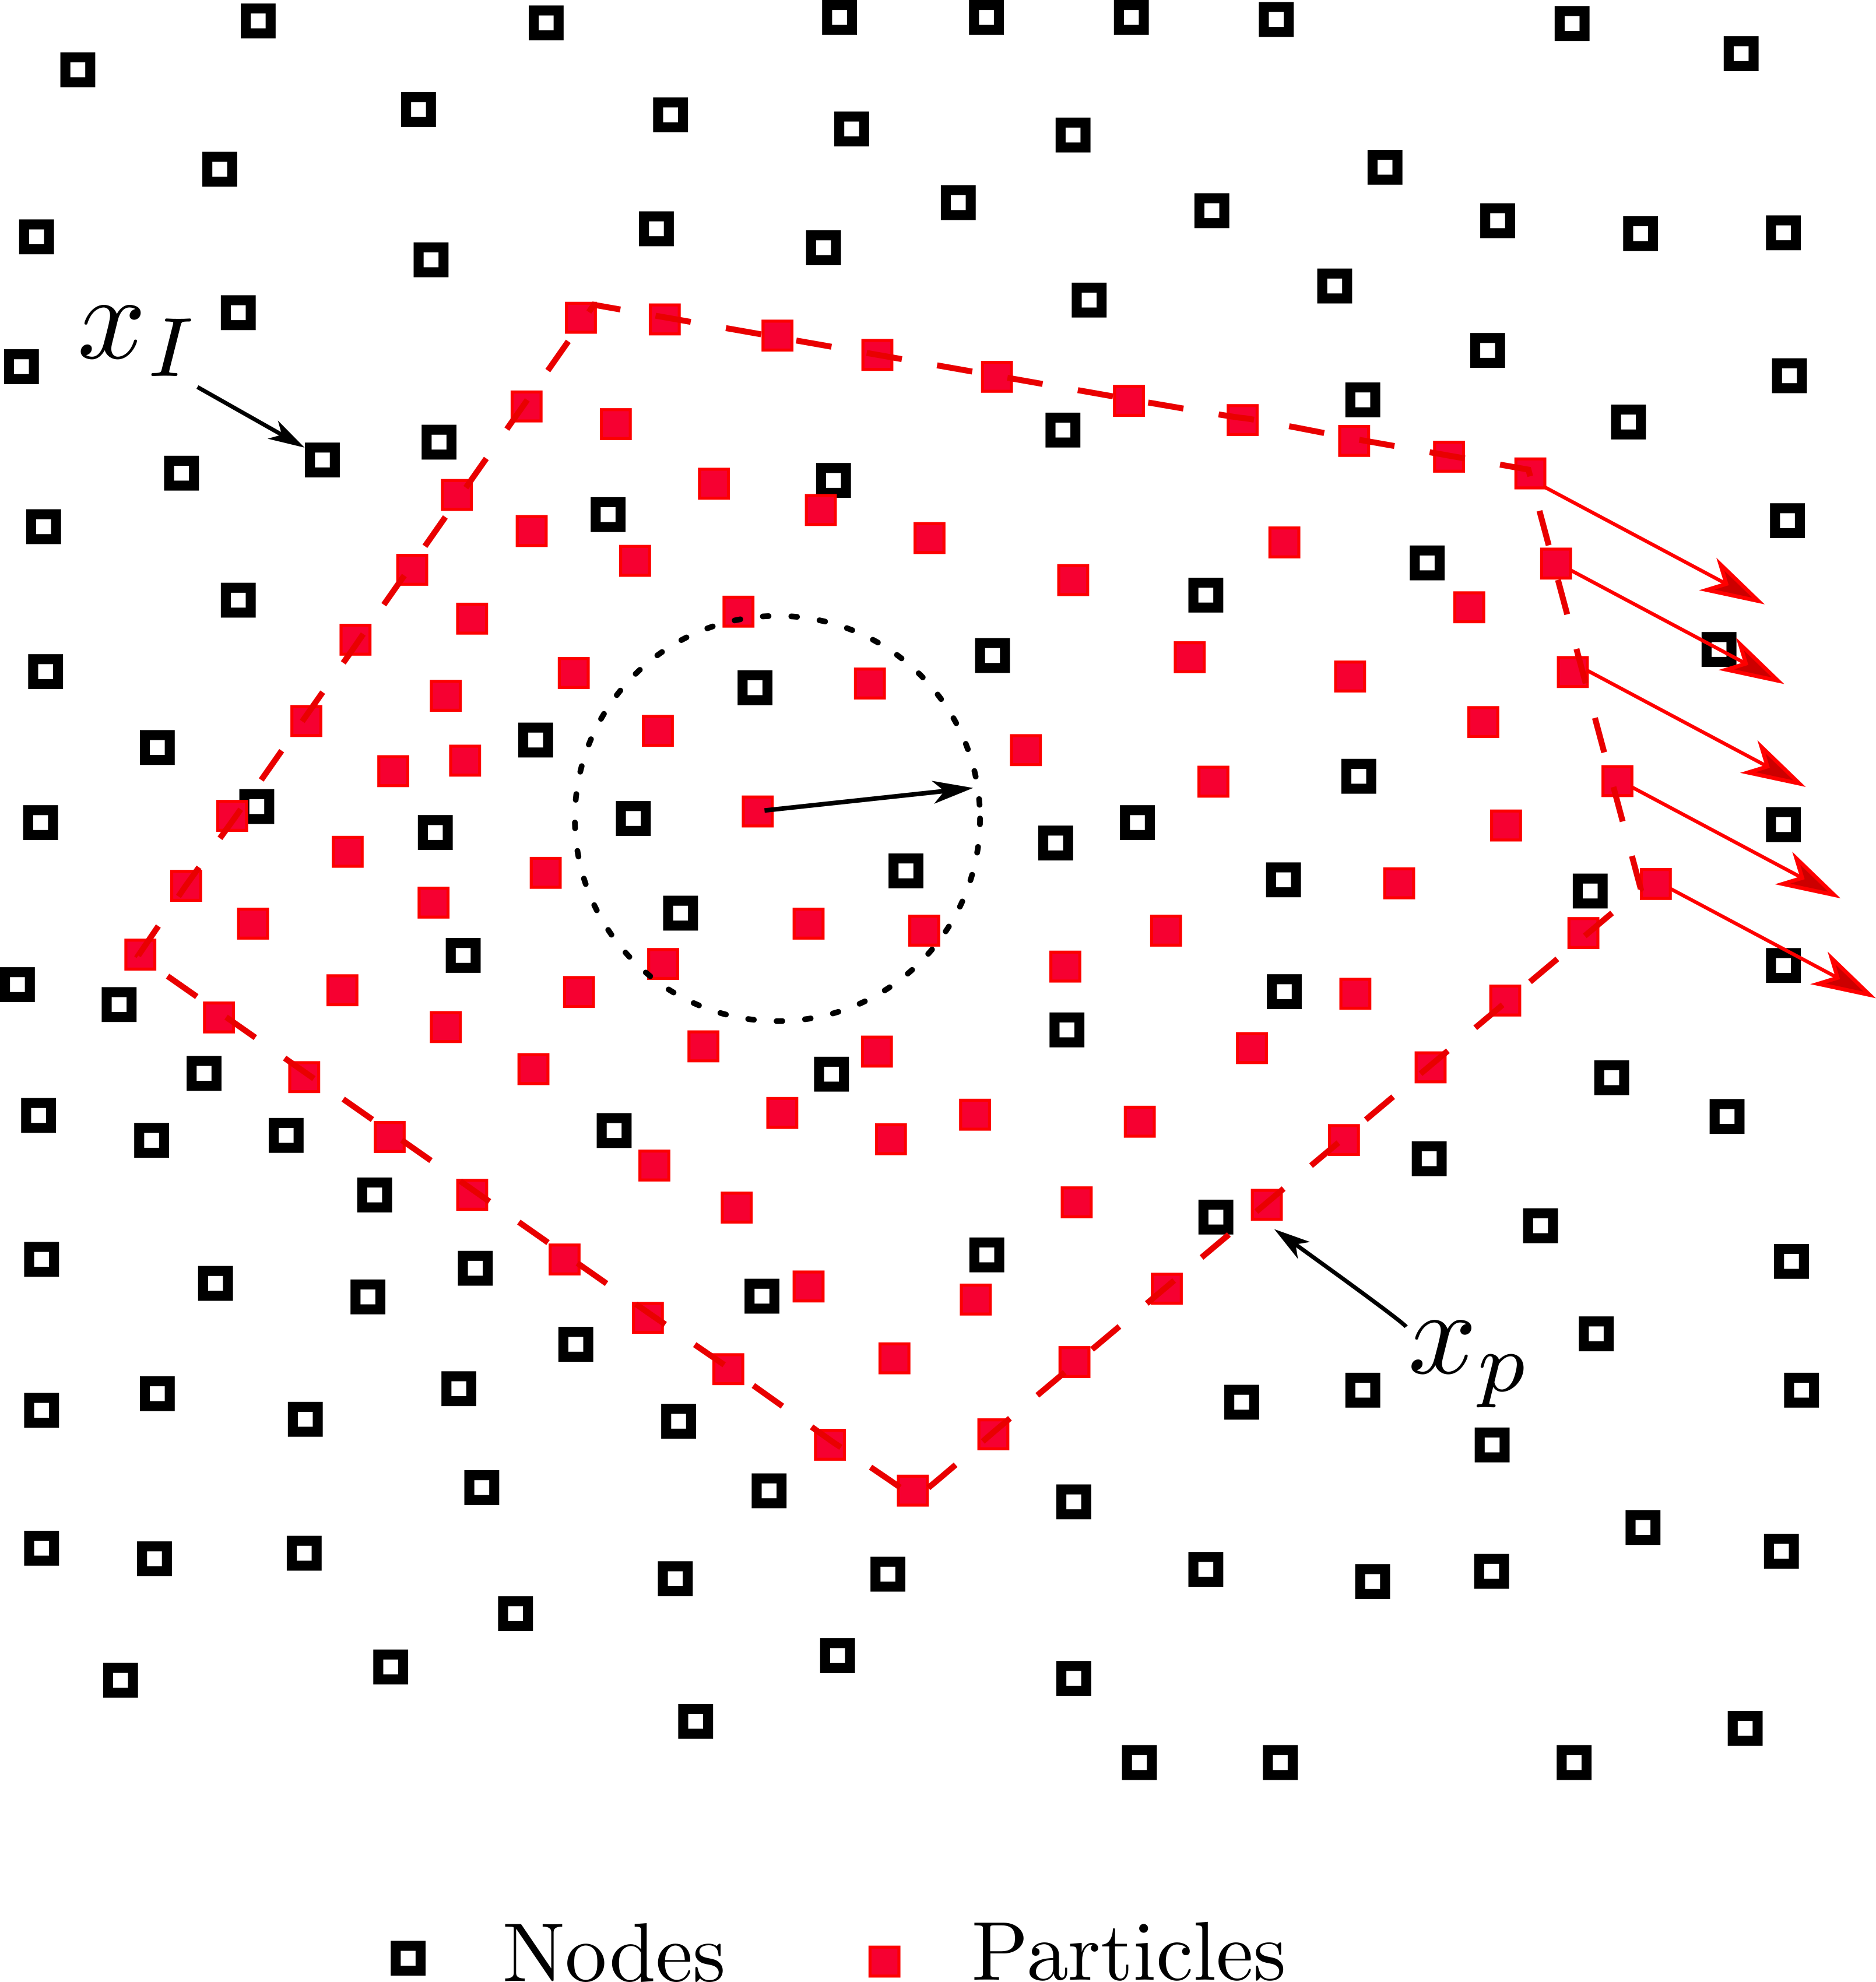
\includegraphics[width=\textwidth]{./Figures/Particle-discretization}
  }
  \caption{This tolerance defines the limit values of the influence
    radius and is used thereafter to find the neighbour nodes of a
    given integration point. The picture also shows the neighbourhood
    criterion to select those node inside of \gls{domain}.} 
  \label{fig:Particle-discretization}
\end{figure}
%%%%%%%%%%%%%%%%%%%%%%%%%%%%%%%%%%%%%%%%%%%%%%%%%%%%%%%%%%%%%%%%%%%%%%%%%%
Due to the \short{fem}-compatibility, the \acrshort{lme} shape function is degenerated to
linear finite element shape function if $d+1$ neighbouring nodes are
chosen as the support. Furthermore, with a conveniently adopted
\textit{regularization} parameter it is possible to get a \acrshort{gimp}-like
shape function. A proof of this statements is observed in figure~\ref{fig:LME_MPM}.  
%%%%%%%%%%%%%%%%%%%%%%%%%%%%%%%%%%%%%%%%%%%%%%%%%%%%%%%%%%%%%%%%%%%%%%%%%%
\begin{figure*}
  \centering
  \subfigure[Q4]{
    \begin{tabular}{c}
      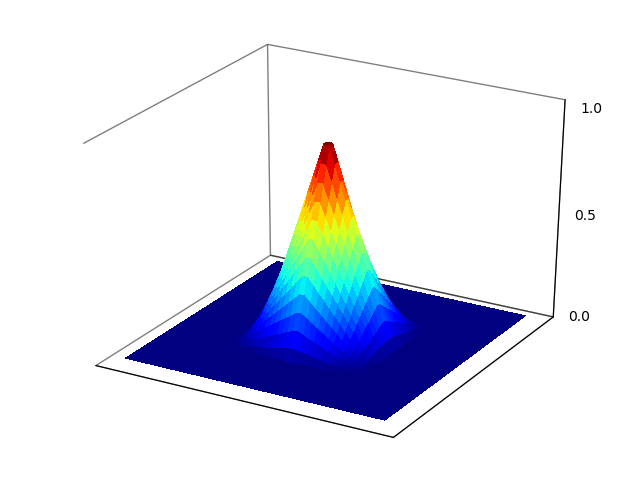
\includegraphics[width=0.14\textwidth]{Figures/MPM_Shape_Fun}\\
      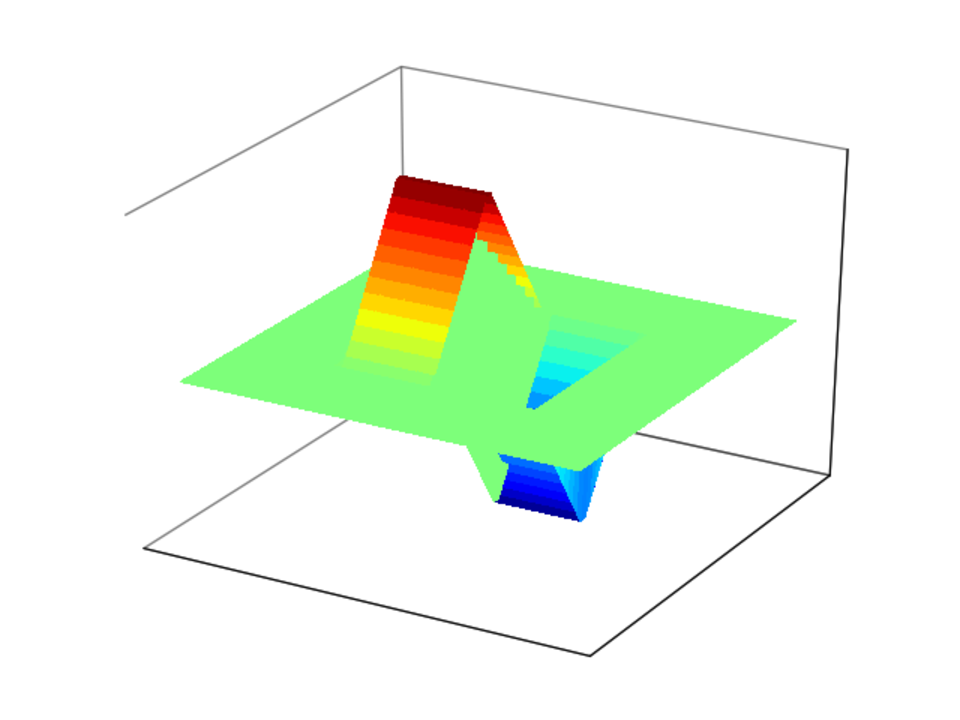
\includegraphics[width=0.14\textwidth]{Figures/MPM_Shape_Fun_dx}\\
      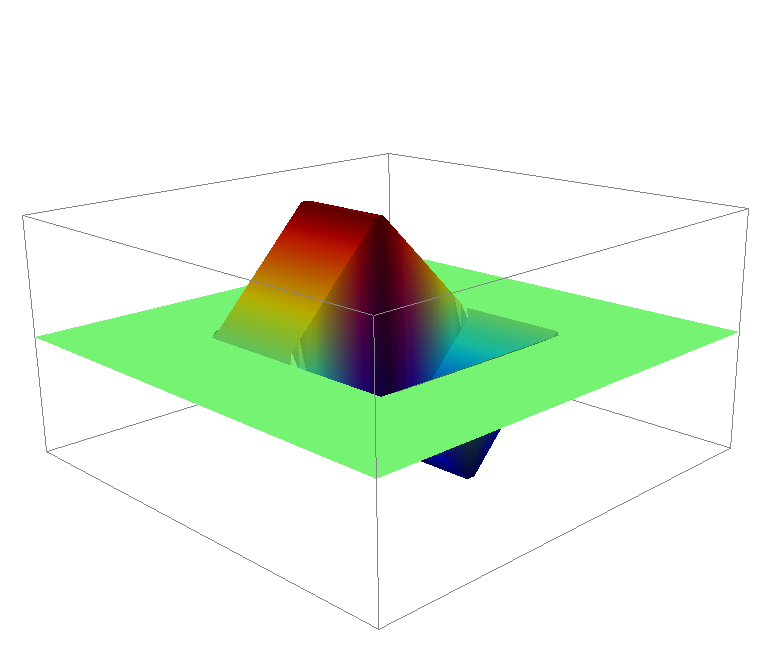
\includegraphics[width=0.14\textwidth]{Figures/MPM_Shape_Fun_dy}
    \end{tabular}  
  }
  \subfigure[$\text{LME}_{17}$]{
    \begin{tabular}{c}
      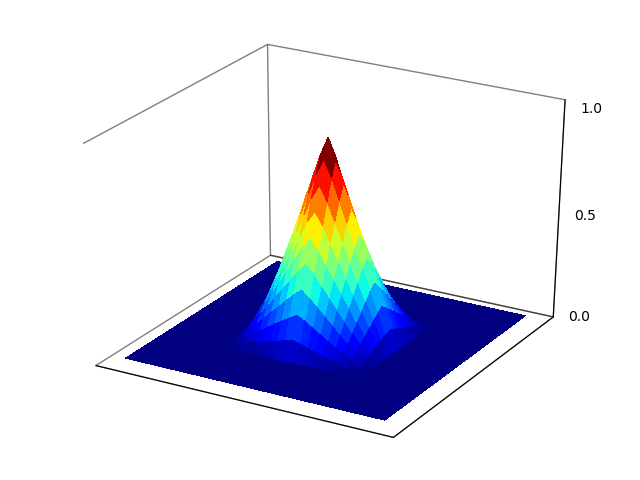
\includegraphics[width=0.14\textwidth]{Figures/LME_17_3_Shape_Fun}\\
      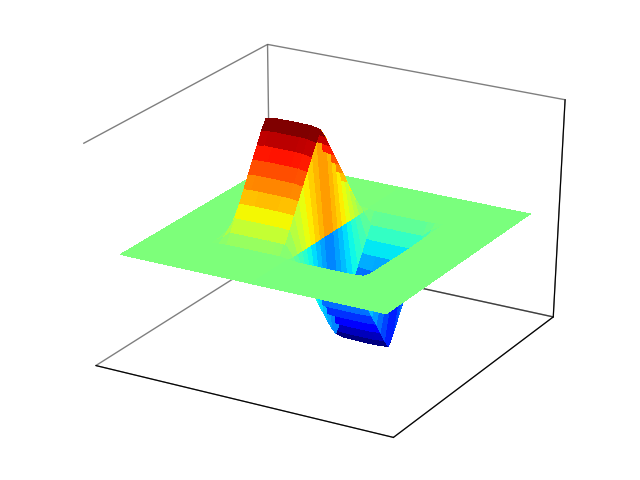
\includegraphics[width=0.14\textwidth]{Figures/LME_17_3_Shape_Fun_dx}\\
      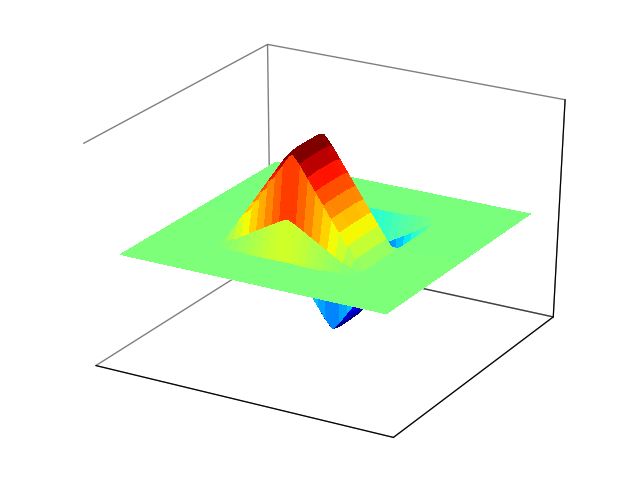
\includegraphics[width=0.14\textwidth]{Figures/LME_17_3_Shape_Fun_dy}
    \end{tabular}
  }
  \subfigure[uGIMP]{
    \begin{tabular}{c}
      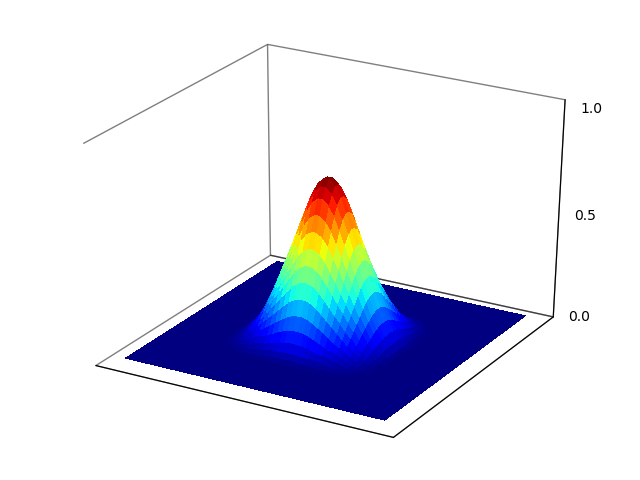
\includegraphics[width=0.14\textwidth]{Figures/GIMP_Shape_Fun}\\
      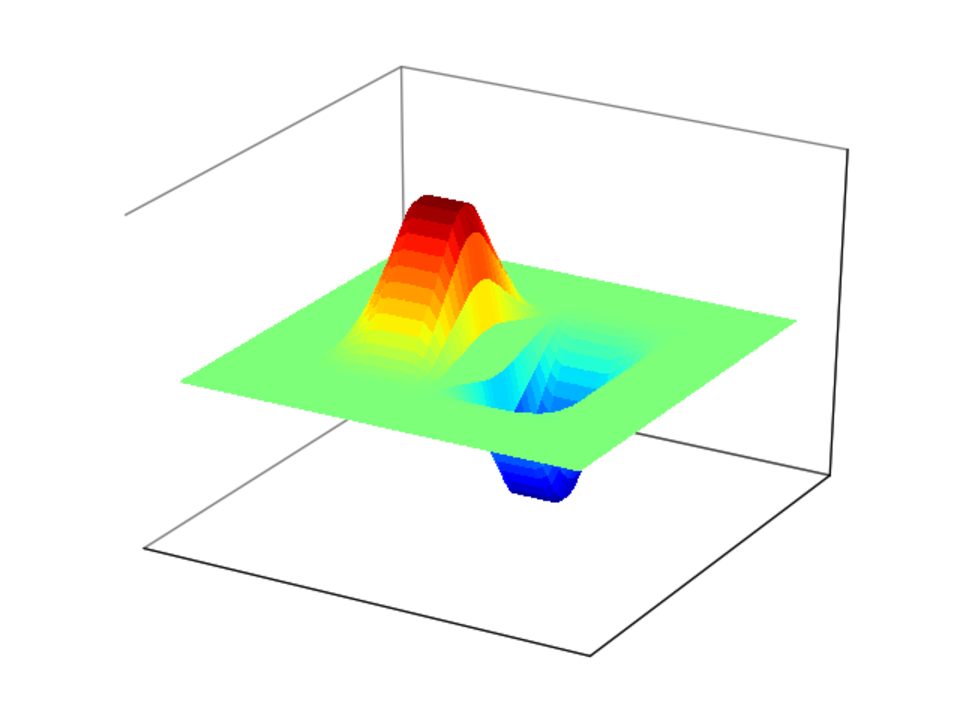
\includegraphics[width=0.14\textwidth]{Figures/GIMP_Shape_Fun_dx}\\
      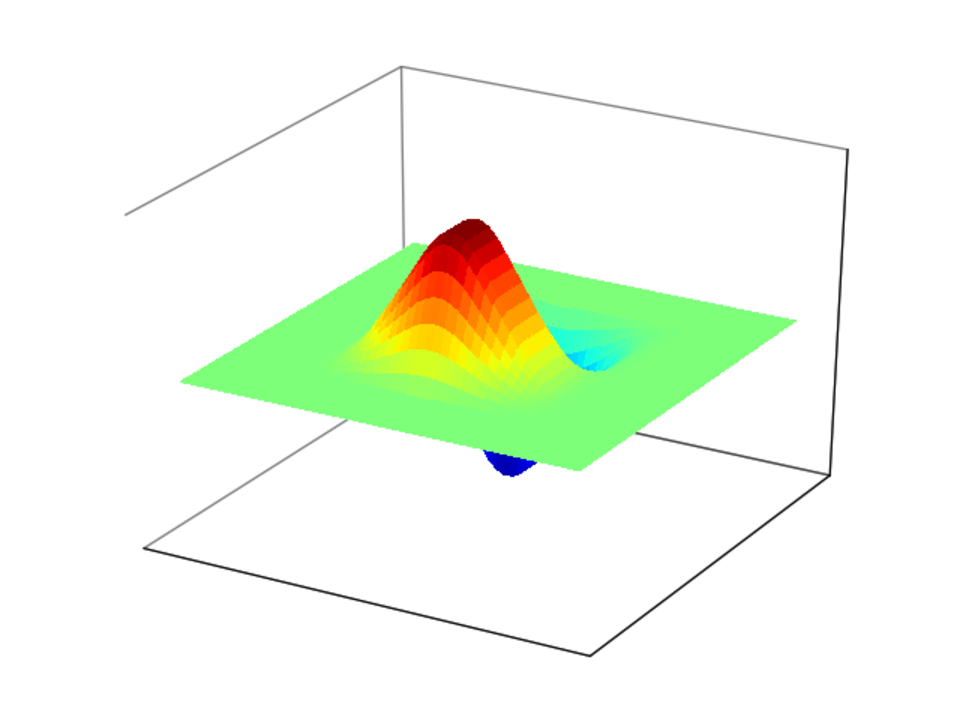
\includegraphics[width=0.14\textwidth]{Figures/GIMP_Shape_Fun_dy}
    \end{tabular}
  }
  \subfigure[$\text{LME}_{10}$]{
    \begin{tabular}{c}
      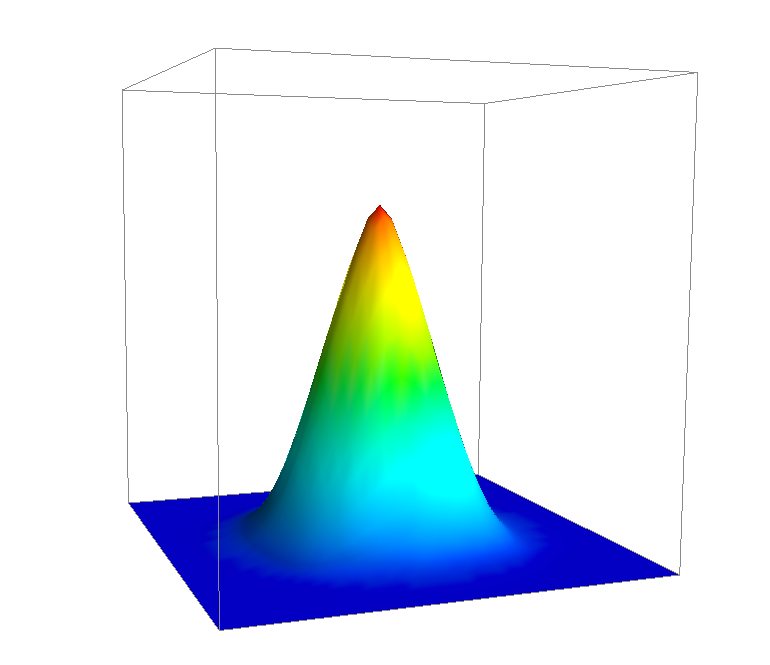
\includegraphics[width=0.14\textwidth]{Figures/LME_10_0_Shape_Fun}\\
      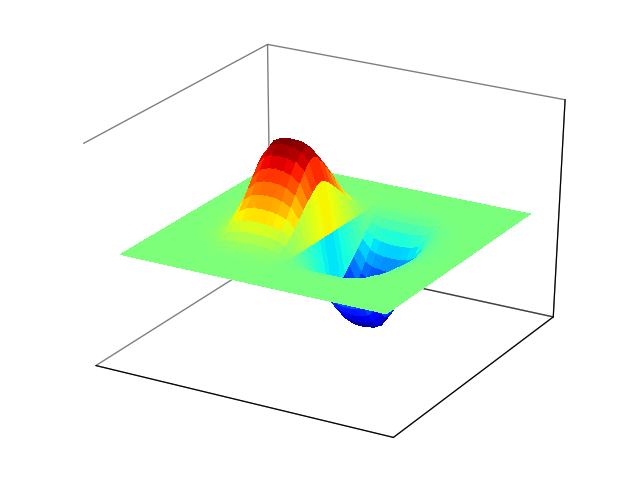
\includegraphics[width=0.14\textwidth]{Figures/LME_10_0_Shape_Fun_dx}\\
      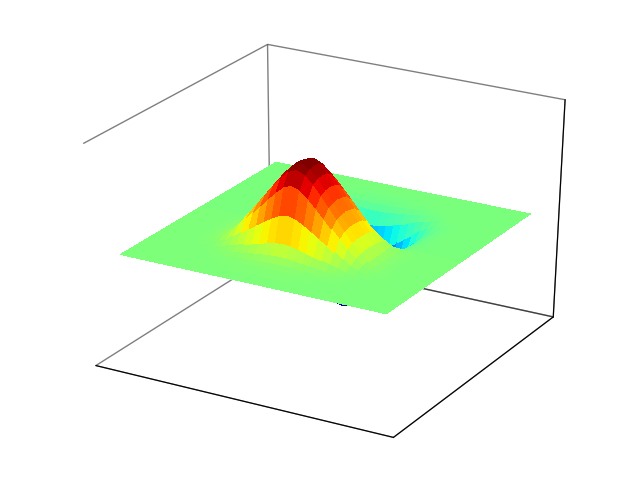
\includegraphics[width=0.14\textwidth]{Figures/LME_10_0_Shape_Fun_dy}    
    \end{tabular}
  }
  \subfigure[$\text{LME}_{5}$]{
    \begin{tabular}{c}
      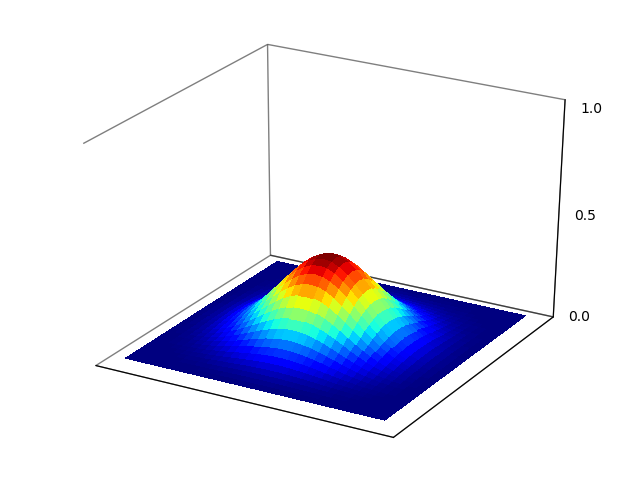
\includegraphics[width=0.14\textwidth]{Figures/LME_5_0_Shape_Fun}\\
      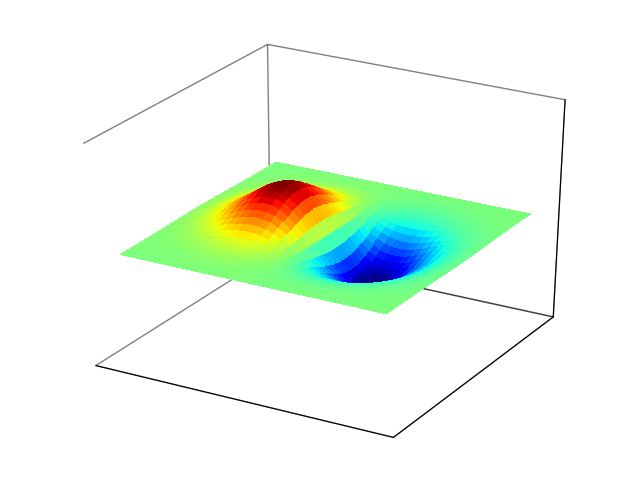
\includegraphics[width=0.14\textwidth]{Figures/LME_5_0_Shape_Fun_dx}\\
      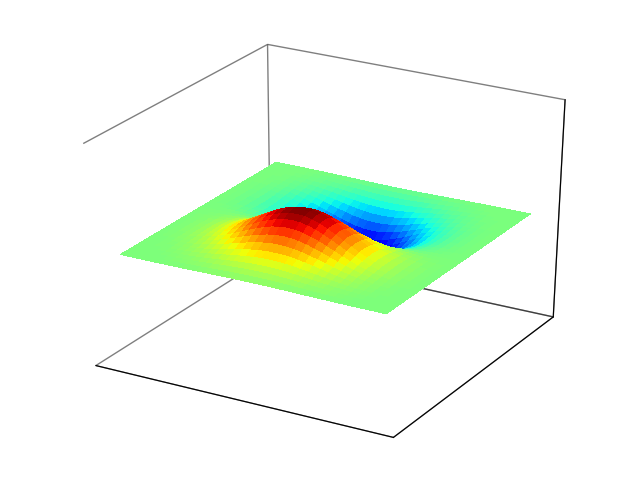
\includegraphics[width=0.14\textwidth]{Figures/LME_5_0_Shape_Fun_dy}
    \end{tabular}
  }
  \caption{Comparative of linear piecewise shape functions (Q4) and
    \acrshort{ugimp} shape functions \textit{versus}  \acrshort{lme}
    approximation for a two-dimensional arrangement of nodes, and
    spatial derivatives for several values of $\gamma = \beta/h^2$.}
  \label{fig:LME_MPM}
\end{figure*}
%%%%%%%%%%%%%%%%%%%%%%%%%%%%%%%%%%%%%%%%%%%%%%%%%%%%%%%%%%%%%%%%%%%%%%%%%%
In this research and in \cite{Arroyo2006}, $\Beta$ is a scalar as the
influence area of the shape function is controlled by the Euclidean
norm, therefore the search area is geometrically a circle in 2D, or a
sphere in 3D. Building upon the idea of anisotropic shape functions,
\cite{Kochmann2019} introduced an enhanced version of the original
\acrshort{lme} scheme, which uses an anisotropic support to deal with 
tensile inestability. Nonetheless this is out of the scope of the
present document but will be incorporated in future research.

\section{Application to linear elasticity dynamic problems.}
\label{sec:Application-linear-elasticity-dynamic-problems}

This section is devoted to test the ability of both predictor-corrector
time integration scheme and the local \textit{max-ent} approximants to
overcome spurious oscillations due to the grid crossing and high
frequency loads under the context of \acrshort{mpm} Two different test has
been adopted for this purpose, the benchmark proposed by Dyka \& Ingel
(1995)\cite{Dyka1995} and the test proposed in the PhD thesis of
Andersen (2009)\cite{thesis_Andersen_2009}. Thought them, the accuracy of the \acrshort{npc}
scheme is compared to the standard \acrshort{fe}. In addition \acrshort{lme} solutions
are compared with those provided by \acrfull{ugimp} and Q4 shape
functions. To avoid some mesh-dependent issues, in all
calculations a regular background mesh was setted. All simulations were performed with in-hose software.

\subsection{Dyka bar \cite{Dyka1995}}
\label{sec:dyka-bar}

This benchmark was proposed due to its ability to shows the capability
of the proposed time integration algorithm to avoid velocity
fields instabilities. It consists in a one-dimensional bar with a
length of 0.1333 meters, sketched in the
figure~\ref{fig:Dyka_Bar}. The boundary conditions are: in the right
border displacement are constrained ($\vect{v} \rvert_{x=L} = 0$) and
in the left displacement are let free ($\tens{\sigma} \rvert_{x=0} =
0$). And a initial velocity of $\vect{v}_o = - 5\ m/s$ is given to the
last quarter of it. Finally, the elastic parameters consider for this test are:
\begin{itemize} 
\item  Density : $7833\ kg/m3$
\item  Poisson ratio : $0$
\item  Elastic modulus : $200 \cdot 10^9\ Pa$
\end{itemize}
%%%%%%%%%%%%%%%%%%%%%%%%%%%%%%%%%%%%%%%%%%%%%%%%%%%%%%%%%%%%%%%%%%%%%%%%%%
\begin{figure}\sidecaption
  \centering
  \resizebox{\hsize}{!}{
    \begin{tikzpicture} 
  \scaling{2}; 
  % Nodos 
  \point{a}{0}{1};
  \point{b}{3.75}{1};
  \point{c}{5}{1};
  % Barras
  \beam{2}{a}{b};
  \beam{2}{b}{c};
  % Apoyos
  \support{3}{a}[270];
  % Fuerzas
  \lineload{4}{b}{c}[1][0.2];
  \notation{5}{b}{c}[$5\ m/s$][.5][below][2];
  % Nombres de nodos
  \notation{1}{a}{A}[below right];
  \notation{1}{b}{B}[below right];
  \notation{1}{c}{C}[below right];
  % Cotas
  \dimensioning{1}{a}{b}{0.5}[{\unit[3/4]{L}}];
  \dimensioning{1}{b}{c}{0.5}[{\unit[1/4]{L}}];
\end{tikzpicture}
}
  \caption{Geometrical description of the Dyka \cite{Dyka1995} bar.}
  \label{fig:Dyka_Bar}
\end{figure}
%%%%%%%%%%%%%%%%%%%%%%%%%%%%%%%%%%%%%%%%%%%%%%%%%%%%%%%%%%%%%%%%%%%%%%%%%%
In this case a duration of 0.0001 seconds for the simulation is
consider. Therefore, the elastic wave generated travel thorough the bar
(from A to C and back to A) at least two times. For the spatial
discretization we adopt a set of seven nodal mesh sizes (0.1, 0.3325, 0.5,
1.0, 3.3325, 6.665, 10.0) in millimeters. For each element a number of
four particles was selected. In the initial layout, particles are
occupying the exact quadrature points of a linear quadrilateral. With
the exception of the \acrshort{ugimp} simulation where gaps or overlap between
voxels of each particle are not allowed. In those cases, each particles
occupy the center of each cell quarter. For all simulations, time step
is controlled by a Courant-Friedrichs-Levy condition of 0.1, were the adopted
celerity is computed as,
\begin{equation}
  \label{eq:Cel}
  Cel = \max\{\max_{p \in \Omega_p}\{ \vect{v}_p \} , \max_{p \in \Omega_p}\{ \sqrt{\frac{E_p}{\rho_p}} \} \}
\end{equation}
A important consideration regarding modellization concerns to the
background mesh. Notice that free border of the bar has a maximum
horizontal displacement of 0.03 millimeters, therefore 
a computational domain with an extra gap of 0.03 millimeters is
required in order to accommodate the unconstrained displacement of the
particles in the left border of the bar. Naturally this problem arise
when the mesh size is small enough that relative displacement of the
particles are larger then the distance to the border, so grid crossing
phenomena could appear even in those cases with infinitesimal
displacements.
%%%%%%%%%%%%%%%%%%%%%%%%%%%%%%%%%%%%%%%%%%%%%%%%%%%%%%%%%%%%%%%%%%%%%%%%%% 
\begin{figure*}\sidecaption
  \centering
  \resizebox{\hsize}{!}{
    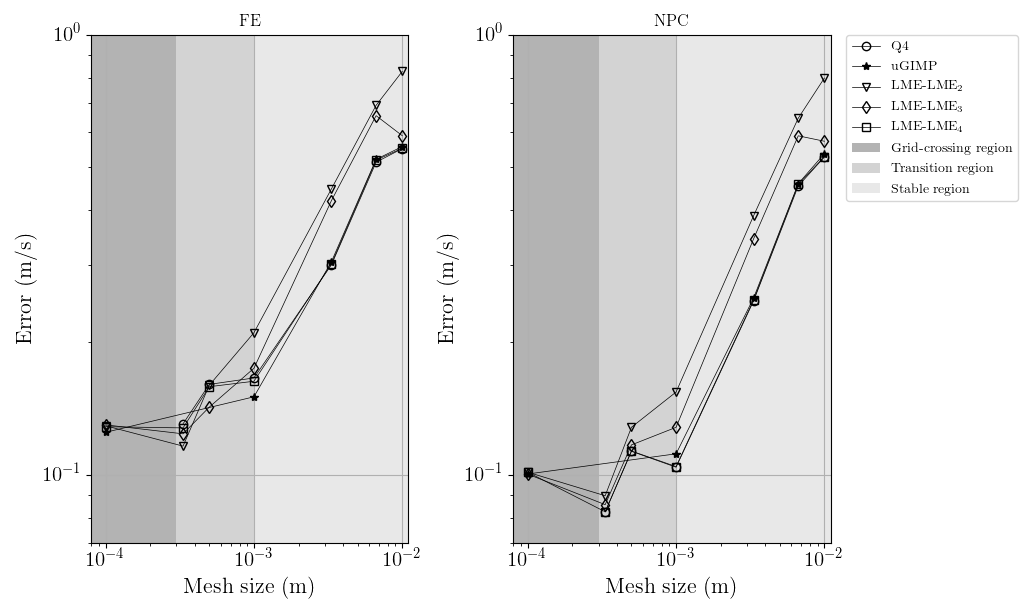
\includegraphics[width=\textwidth]{./Figures/Error_evol}
  }
  \caption{Velocity evolution at the point in the Dyka bar left side,
    convergence plots for \acrshort{fe} and \acrshort{npc}. The plot is subdivided with
    colours, the darker part of the diagram shows coincides when the
    relative movement of the particles is large enough to produce the
    grid crossing phenomena. The lightest part of the diagram
    coincides when the relative movement of the particles in
    negligible in comparison with the mesh size. And in the middle
    region a transition behaviour take place.}
  \label{fig:Dyka-error-evol}
\end{figure*}
%%%%%%%%%%%%%%%%%%%%%%%%%%%%%%%%%%%%%%%%%%%%%%%%%%%%%%%%%%%%%%%%%%%%%%%%%%
In this case, an analytical solution is possible
thought the characteristics method described in the appendix
\ref{app:analytical_sol}. To measure the convergence of the solutions
for the different time integration and approximation schemes the
root-mean-square (RMS) error in the velocity field is computed. RMS
error is defined as
\begin{equation}
  \label{eq:RMS}
  RMS = \sqrt{\frac{1}{N} \sum^{N}_p \left( \vect{v}_p - \hat{\vect{v}}_p \right)^2},
\end{equation}
where $\vect{v}_p$ and $\hat{\vect{v}}_p$ are respectively the analytical and
numerical solutions evaluated in the final time step in the position
of each particle. A first comparative between both time integration
scheme is plotted in figure \ref{fig:Dyka-NPC-FE}. It demonstrates the
superior performance of the \acrshort{npc} \textit{versus} the \acrshort{fe}. In the \acrshort{npc} the
spurious oscillations are quickly mitigated in the first time steps,
and does not propagate the error in time in opposite to \acrshort{fe} where the
simulation becomes unstable after $6E^{5}$ seconds. Figure
\ref{fig:Dyka-error-evol} also remarks the remarkable difference
between both schemes. 
%%%%%%%%%%%%%%%%%%%%%%%%%%%%%%%%%%%%%%%%%%%%%%%%%%%%%%%%%%%%%%%%%%%%%%%%%%
\begin{figure}\sidecaption
  \centering
  \resizebox{0.9\hsize}{!}{
    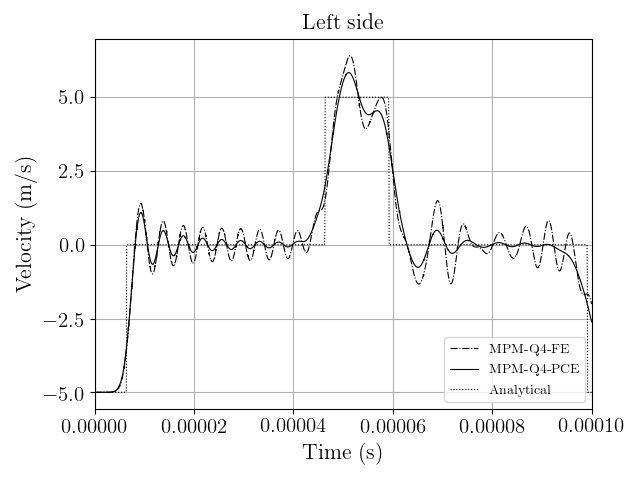
\includegraphics[width=\textwidth]{./Figures/Velocity_FE_vs_PCE_CFL_01}
  }
  \caption{Comparative of the \acrshort{npc} \textit{versus} the \acrshort{fe}. In the
    picture the velocity evolution at the point in the bar left side
    is plotted.}
  \label{fig:Dyka-NPC-FE}
\end{figure}
%%%%%%%%%%%%%%%%%%%%%%%%%%%%%%%%%%%%%%%%%%%%%%%%%%%%%%%%%%%%%%%%%%%%%%%%%%
Figure \eqref{fig:Dyka-LME-gamma} shows the sensibility of the \acrshort{lme}
approximation scheme to variations in the a-dimensional parameter
$\beta$ that controls the value of the regularization parameter
$\gamma$ depending of the mesh size. Notice how lower values of
gamma exhibits a behaviour with a soft decay in some parts of the
simulation due to the increase of nodes adopted to regularize the
solutions. This capability could be useful in simulations where
extremely noise oscillations could damage the solutions like memory
materials. On the other hand larger values of the parameter $\beta$
makes the solution tend to the linear \acrshort{fem} solution as the athermal
limit is reached \cite{Arroyo2006}. Intermediate values of the
regularization parameters give us a compromise between the both
scenarios here described. An additional observation concerning the
solution sensibility to regularization parameters occurs when mesh
size decreases. For larger mesh size where the relative particle displacement
is negligible in comparison with the cell size, the global behaviour
is \acrshort{fem}-like, therefore larger values of $\gamma$ has offers better
results. On the other hand, when mesh size is small enough to produce
grid-crossing and mesh-free behaviour is required to ensures the
convergence of the solution, tiny values of $\gamma$ has a better
performance. Convergence plot in figure \eqref{fig:Dyka-error-evol}
shows how the slope for the larger values of $\gamma$ decreases
monotonically with the value of the mesh size, in contrast to larger
values of it, whose suffers a punishment of the performance when significant
movement of the particles occurs as far mesh size is reduced.  
%%%%%%%%%%%%%%%%%%%%%%%%%%%%%%%%%%%%%%%%%%%%%%%%%%%%%%%%%%%%%%%%%%%%%%%%%%
\begin{figure}\sidecaption
  \centering
  \resizebox{0.9\hsize}{!}{
    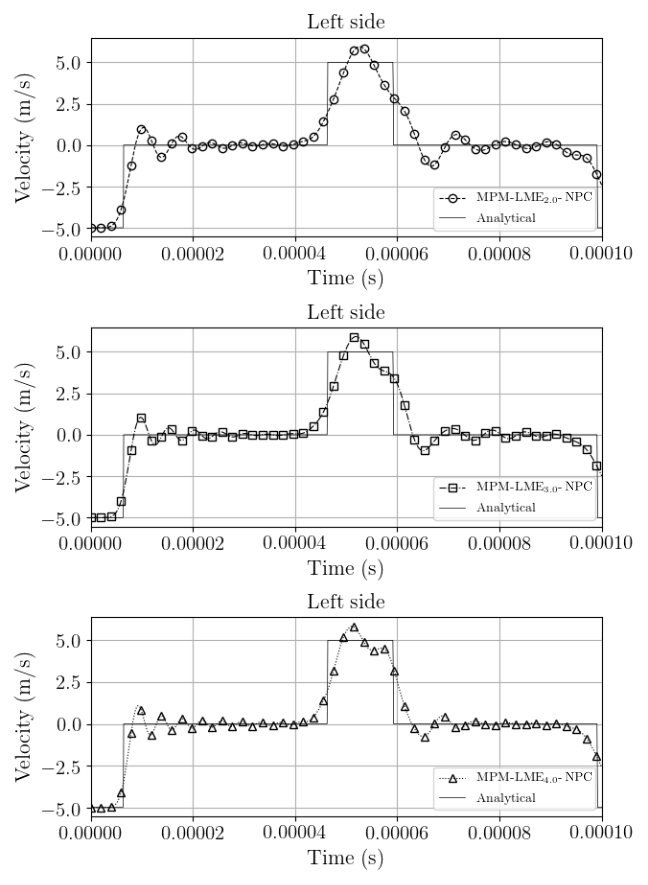
\includegraphics[width=\textwidth]{./Figures/Velocity_LME_gamma_comparative}
  }
  \caption{Sensitive of LME approximants performance to changes in the
    adimensional regularization parameter $\gamma = \beta/h^2$. To
    illustrate it, the velocity evolution at the point in the bar left side
    is plotted.}
  \label{fig:Dyka-LME-gamma}
\end{figure}
%%%%%%%%%%%%%%%%%%%%%%%%%%%%%%%%%%%%%%%%%%%%%%%%%%%%%%%%%%%%%%%%%%%%%%%%%%
Figure \ref{fig:Dyka-uGIMP-LME} compares the performance of the
\acrshort{ugimp}~\cite{Bardenhagen2004} shape function \textit{versus} the \acrshort{lme} approximation scheme with
a adimensional regularization parameter $\gamma$ of 4.0. Although it
does not shows remarkable differences, \acrshort{lme} approximats exhibits a more
robust behaviour than the \acrshort{ugimp} shape functions. Regarding this, notice
the absence of \acrshort{ugimp} values for a mesh size of 0.3325 and 0.5
millimeters. This is because during these simulation the \acrshort{ugimp} suffered an unstable
increase of the error which yield unacceptable results. A feasible
explanation for this phenomena could be the presence of numerical
cancellation which could produce gaps between voxels. Further research
should be done in this direction for getting a better comprehension of
this phenomena. In opposite, \acrshort{lme} approximation does not
suffers this phenomena either with irregular nodal layout.
%%%%%%%%%%%%%%%%%%%%%%%%%%%%%%%%%%%%%%%%%%%%%%%%%%%%%%%%%%%%%%%%%%%%%%%%%%
\begin{figure}\sidecaption
  \centering
  \resizebox{0.9\hsize}{!}{
    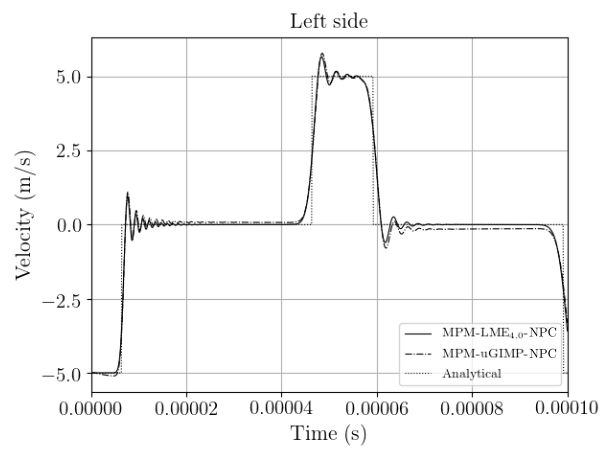
\includegraphics[width=\textwidth]{./Figures/Velocity_uGIMP_vs_LME_Dyka}
  }
  \caption{Velocity evolution at the point in the bar left side.}
  \label{fig:Dyka-uGIMP-LME}
\end{figure}
%%%%%%%%%%%%%%%%%%%%%%%%%%%%%%%%%%%%%%%%%%%%%%%%%%%%%%%%%%%%%%%%%%%%%%%%%%
Finally, figure \ref{fig:Dyka-OTM-MPM} compares the solution obtained
with \acrshort{otm}~\cite{Li2010} \textit{versus} the solution obtained with \acrshort{mpm},
both with same time integration scheme and spatial discretization. For
this case the performance of \acrshort{mpm} is robust and stable than
\acrshort{otm}. During the first half of the simulation both method 
seem to perform in a similar way, but during the second half of the
simulation after the elastic wave has travel from the free border to
the fixed one and back, in \acrshort{otm} the solution becomes noisy than the
one performed by \acrshort{mpm}.  
%%%%%%%%%%%%%%%%%%%%%%%%%%%%%%%%%%%%%%%%%%%%%%%%%%%%%%%%%%%%%%%%%%%%%%%%%%
\begin{figure}\sidecaption
  \centering
  \resizebox{0.9\hsize}{!}{
    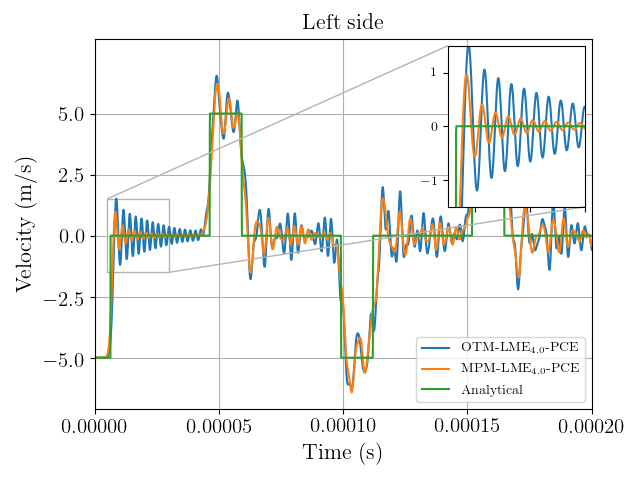
\includegraphics[width=\textwidth]{./Figures/Velocity_MPM_vs_OTM_Dyka}
  }
  \caption{Velocity evolution at the point in the bar left side.}
  \label{fig:Dyka-OTM-MPM}
\end{figure}
%%%%%%%%%%%%%%%%%%%%%%%%%%%%%%%%%%%%%%%%%%%%%%%%%%%%%%%%%%%%%%%%%%%%%%%%%%

\subsection{Andersen block}
\label{sec:andersen-block}

The following test was proposed to measure proof the ability of this
interpolation technique to deal with grid crossing instabilities. It
consists in the simulation of a square block of soil incrementally
loaded by a body force. Details of the problem are sketched in figure~\ref{fig:block}
%%%%%%%%%%%%%%%%%%%%%%%%%%%%%%%%%%%%%%%%%%%%%%%%%%%%%%%%%%%%%%%%%%%%%%%%%%
\begin{figure}\sidecaption
  \centering
  \resizebox{0.7\hsize}{!}{
    \begin{tikzpicture} 
  \scaling{1};
  
% Nodos
\point{1}{0}{10};
\point{2}{2}{10};
\point{3}{0}{8};
\point{4}{2}{8};
\point{5}{4}{10};
\point{6}{0}{6};
\point{7}{2}{6};
\point{8}{4}{8};
\point{9}{4}{6};
\point{10}{6}{10};
\point{11}{0}{4};            
\point{12}{2}{4};            
\point{13}{6}{8};            
\point{14}{4}{4};            
\point{15}{6}{6};            
\point{16}{8}{10};            
\point{17}{0}{2};            
\point{18}{2}{2};            
\point{19}{8}{8};            
\point{20}{6}{4};            
\point{21}{4}{2};            
\point{22}{8}{6};            
\point{23}{0}{0};            
\point{24}{10}{10};            
\point{25}{6}{2};            
\point{26}{8}{4};
\point{27}{2}{0};            
\point{28}{10}{8};            
\point{29}{4}{0};            
\point{30}{10}{6};            
\point{31}{8}{2};            
\point{32}{6}{0};            
\point{33}{10}{4};            
\point{34}{8}{0};            
\point{35}{10}{2};            
\point{36}{10}{0};

% Barras
\beam{2}{27}{18};
\beam{2}{18}{17};
\beam{2}{17}{23};
\beam{2}{23}{27};
  
\beam{2}{29}{21};
\beam{2}{21}{18};
\beam{2}{18}{27};
\beam{2}{29}{27};

\beam{2}{32}{25};
\beam{2}{25}{21};
\beam{2}{21}{29};
\beam{2}{32}{29};

\beam{2}{34}{31};
\beam{2}{31}{25};
\beam{2}{25}{32};
\beam{2}{34}{32};

\beam{2}{36}{35};
\beam{2}{35}{31};
\beam{2}{31}{34};
\beam{2}{36}{34};

%%%%%%%%%%%%%%%%
\beam{2}{18}{12};
\beam{2}{12}{11};
\beam{2}{11}{17};
\beam{2}{18}{17};

\beam{2}{21}{14};
\beam{2}{14}{12};
\beam{2}{12}{18};
\beam{2}{21}{18};

\beam{2}{25}{20};
\beam{2}{20}{14};
\beam{2}{14}{21};
\beam{2}{25}{21};

\beam{2}{31}{26};
\beam{2}{26}{20};
\beam{2}{20}{25};
\beam{2}{31}{25};

\beam{2}{35}{33};
\beam{2}{33}{26};
\beam{2}{26}{31};
\beam{2}{35}{31};

%%%%%%%%%%%%%%%%
\beam{2}{12}{7};
\beam{2}{7}{6};
\beam{2}{6}{11};
\beam{2}{12}{11};

\beam{2}{14}{9};
\beam{2}{9}{7};
\beam{2}{7}{12};
\beam{2}{14}{12};

\beam{2}{20}{15};
\beam{2}{15}{9};
\beam{2}{9}{14};
\beam{2}{20}{14};

\beam{2}{26}{22};
\beam{2}{22}{15};
\beam{2}{15}{20};
\beam{2}{26}{20};

\beam{2}{33}{30};
\beam{2}{30}{22};
\beam{2}{22}{26};
\beam{2}{33}{26};

%%%%%%%%%%%%%%%%
\beam{2}{7}{4};
\beam{2}{4}{3};
\beam{2}{3}{6};
\beam{2}{7}{6};

\beam{2}{9}{8};
\beam{2}{8}{4};
\beam{2}{4}{7};
\beam{2}{9}{7};

\beam{2}{15}{13};
\beam{2}{13}{8};
\beam{2}{8}{9};
\beam{2}{15}{9};

\beam{2}{22}{19};
\beam{2}{19}{13};
\beam{2}{13}{15};
\beam{2}{22}{15};

\beam{2}{30}{28};
\beam{2}{28}{19};
\beam{2}{19}{22};
\beam{2}{30}{22};

%%%%%%%%%%%%%%%%
\beam{2}{4}{2};
\beam{2}{2}{1};
\beam{2}{1}{3};
\beam{2}{4}{3};

\beam{2}{8}{5};
\beam{2}{5}{2};
\beam{2}{2}{4};
\beam{2}{8}{4};

\beam{2}{13}{10};
\beam{2}{10}{5};
\beam{2}{5}{8};
\beam{2}{13}{8};

\beam{2}{19}{16};
\beam{2}{16}{10};
\beam{2}{10}{13};
\beam{2}{19}{13};

\beam{2}{28}{24};
\beam{2}{24}{16};
\beam{2}{16}{19};
\beam{2}{28}{19};

% Bottom
\support {1}{23}[315];
\support {1}{27}[0];
\support {1}{29}[0];
\support {1}{32}[0];
\support {1}{34}[0];
\support {1}{36}[45];

% \support {2}{23}[270];
\support {2}{1}[270];
\support {2}{3}[270];
\support {2}{6}[270];
\support {2}{11}[270];
\support {2}{17}[270];

\support {2}{24}[90];
\support {2}{28}[90];
\support {2}{30}[90];
\support {2}{33}[90];
\support {2}{35}[90];
% \support {2}{36}[90];

% Gravity
\point{g}{12}{5};
\load{1}{g}[90][3][0];

% Cotas
\dimensioning{1}{23}{36}{-1.5}[$10~m$];
\dimensioning{2}{23}{1}{-1.5}[$10~m$];


\end{tikzpicture}


% % Apoyos
% \support{3}{c}[90];
% % Fuerzas
% \lineload{4}{b}{a}[1][0.2];
% \notation{5}{a}{b}[$-5\ m/s$][.5][below][2];
% % Nombres de nodos
% \notation{1}{a}{A}[below left];
% \notation{1}{b}{B}[below left];
% \notation{1}{c}{C}[below left];
% % Cotas
% \dimensioning{1}{a}{b}{0.5}[{\unit[1/4]{L}}];
% \dimensioning{1}{b}{c}{0.5}[{\unit[3/4]{L}}];


% End Elements
}
  \caption{Geometrical description of a soil block }.}
  \label{fig:block}
\end{figure}
%%%%%%%%%%%%%%%%%%%%%%%%%%%%%%%%%%%%%%%%%%%%%%%%%%%%%%%%%%%%%%%%%%%%%%%%%%
This test was taken from PhD thesis of Andersen (2009)\cite{thesis_Andersen_2009}. The
elastic parameters consider for this test are: 
\begin{itemize} 
\item  Initial density : $6\cdot 10^3\ kg/m^3$
\item  Poisson ratio : $0$
\item  Elastic modulus : $5\ MPa$
\end{itemize}
The gravity force is a apply as an external force according to the
equations \eqref{eq:particle_body_forces},
\eqref{eq:nodal_external_forces}. Using a total time period of T (20
seconds) to apply the gravity, it is increased from 0 to 9.81$m/s$
with a sinus function until T/2 and then maintained constant until T
in order to arrive to a state of equilibrium, 
\begin{equation}
  \label{eq:gravity-load-block}
 \mathbf{g}(t) = \left\{
    \begin{array}{ll}
      0.5 \mathbf{g} (\sin(\frac{2t \pi}{T} - \frac{\pi}{2})+1)  & \mbox{if } t \leq T/2 \\
      \mathbf{g} & \mbox{if } t > T/2
    \end{array}
  \right.
\end{equation}
In order to get a stable solution, time step was conducted by a
Courant number of 0.1. On the other hand, the explicit
predictor-corrector scheme is here employed looking forward getting better results. For the
initial spatial discretization four particles per cell
($\Delta x = 2\ m$) were adopted. The initial layout of particles inside of the
cell changes according to the approximation technique adopted. For the
bi-linear shape functions and the \acrshort{lme} approximants, the initial
position corresponds to the location of the gauss-points in a standard
quadratic finite element. For the \acrshort{ugimp} shape function the initial
position of each particle is located in the center of each voxel, due
to the fact that in the initial situation, the voxel domain should not
overlap each others.

Figure~\ref{fig:Block-LME3} shows the evolution of the vertical stress
during the loading process. The result is physically realistic as
stress increments linearly from the top to the bottom of the specimen,
and the value of the vertical stress in a material point located in
the bottom of the specimen oscillates centered in $5.2 MPa$, which is
the analytic value given by $\sigma_{yy} = \rho g h_y$.
%%%%%%%%%%%%%%%%%%%%%%%%%%%%%%%%%%%%%%%%%%%%%%%%%%%%%%%%%%%%%%%%%%%%%%%%%%
\begin{figure*}
  \centering
  \subfigure[t = 0 seconds.]{
    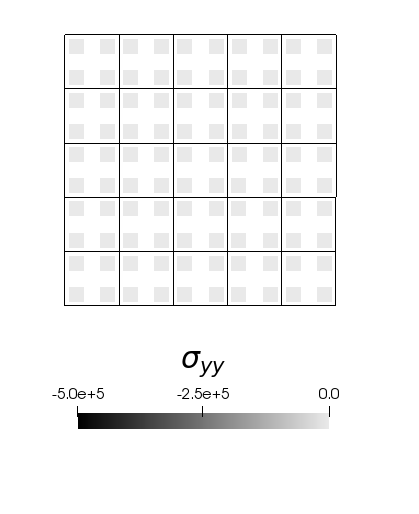
\includegraphics[width=0.3\textwidth]{Figures/Block_LME3_PCE_a_t0}
  }
  \subfigure[t = 5 seconds.]{
    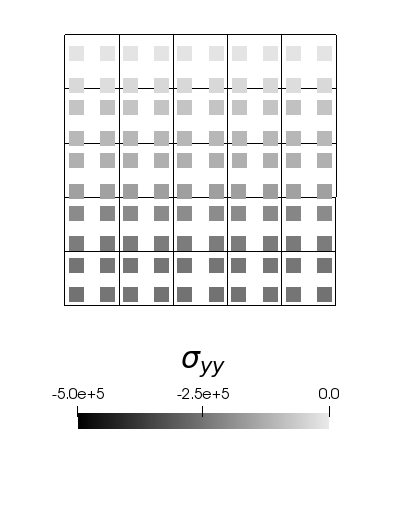
\includegraphics[width=0.3\textwidth]{Figures/Block_LME3_PCE_b_t025}
  }
  \subfigure[t = 20 seconds]{
    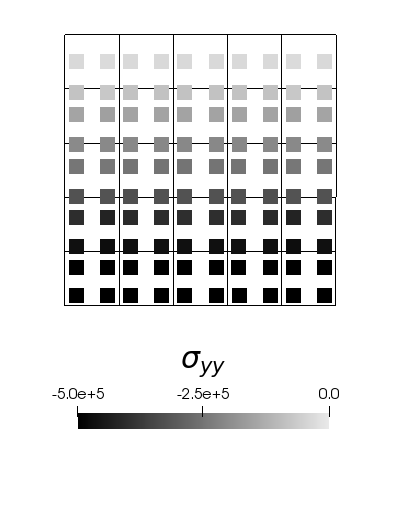
\includegraphics[width=0.3\textwidth]{Figures/Block_LME3_PCE_c_t1}
  }
  \caption{Vertical normal stress and position of material points
    during the loading process for a soft soil ($E = 5\ MPa$, $\rho_0
    = 6\cdot 10^3\ kg/m^3$). Numerical parameters considered for the
    simulation are : Local \textit{max-ent} shape function $\gamma =3$
    and explicit PC scheme with CFL 0.1.}
  \label{fig:Block-LME3}
\end{figure*}
%%%%%%%%%%%%%%%%%%%%%%%%%%%%%%%%%%%%%%%%%%%%%%%%%%%%%%%%%%%%%%%%%%%%%%%%%%
Figure~\ref{fig:vertical-displacement-block} shows the vertical
displacement evolution of a point in the free surface of the
block. This figure shows how simulations performed with a bi-linear
interpolation technique (Q4) turns out to be unstable during
cell-crossing and consequently fails. The \acrshort{ugimp} simulation
is more stable than the one performed by the Q4. Despite this is still
unstable and could trigger severe oscillations in simulation with
non-linear  materials. The \acrshort{lme} simulation was performed
using two kinds of shape functions, one with a low value of the
dimensionless parameter, $\gamma = 0.8$, and other with a larger value
of it, $\gamma = 3.0$. Notice that the results are both stable, but
the larger values of $\gamma$ give us a very stable solution. This is
due to the fact that with larger value of $\gamma$, the shape
functions behaves in a similar way to the \acrshort{fem}, which performs very
accurate in those cases with a reasonable mesh distorsion, and with a
lower value it behaves in a similar way to the \acrshort{ugimp}. This behaviour
was noticed previously by \cite{Arroyo2006}, were authors highlight
how by adjusting the spatial variation of $\beta(\vect{x})$, it is
possible to select regions of the domain of analysis which are treated
by finite elements and regions that are treated in the style of
meshfree methods, with seamless transitions between those regions. 
%%%%%%%%%%%%%%%%%%%%%%%%%%%%%%%%%%%%%%%%%%%%%%%%%%%%%%%%%%%%%%%%%%%%%%%%%%
\begin{figure}\sidecaption
  \centering
  \resizebox{\hsize}{!}{
    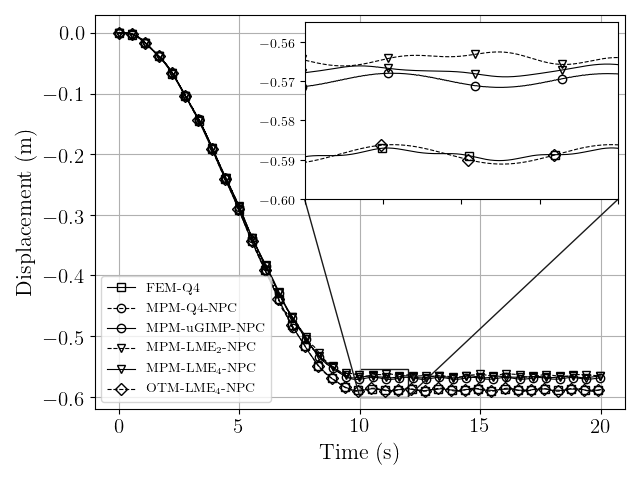
\includegraphics[width=\textwidth]{./Figures/Block_CFL_01_Comparative}
  }
  \caption{Comparative of the vertical displacement evolution in a
    point located in the free surface employing different
    interpolation schemes and numerical techniques.} 
  \label{fig:vertical-displacement-block}
\end{figure}
%%%%%%%%%%%%%%%%%%%%%%%%%%%%%%%%%%%%%%%%%%%%%%%%%%%%%%%%%%%%%%%%%%%%%%%%%%


\section{Conclusions}
\label{sec:conclusions}
We have developed a novel time integration scheme for \acrshort{mpm}, and
proved how local \textit{max-ent} approximation scheme could be
employed as an useful technique in \acrshort{mpm}. The \acrshort{npc} arise as a highly
efficient alternative for challenging dynamic problems like coupled
$u-p_w$ without appeal to expensive implicit time integration
algorithms. Also the procedure employed to design the \acrshort{npc} algorithm open
the door to revisit a huge variety of time integration schemes
developed originally for \acrshort{fem}, which can be rearranged to \acrshort{mpm} framework
with some modifications. Anyway, further research should be done to improve the
formal comprehension of the algorithm good performance. This paper
also enhances the suitability of the \acrshort{lme} approximation as a
general promising alternative to the wide range of approximation.
techniques developed for the \acrshort{mpm} to overcome grid crossing
limitations and to avoid the constriction of the \acrshort{ugimp} of a regular mesh
or a high density of particles per cell. Future research of the
group will be on the employ of this scheme to improve the localization
capabilities of \acrshort{mpm} for viscoplastic materials. Finally we remark on
the possibility of adapting the function $\beta(\vect{x})$ as a second
order tensor with the aim of adapt the shape function with the strain field which improves the
performance of it in the aforementioned localization
capabilities. Other possibility is to adapt the value of $\beta$ to
solve the equations \acrshort{fem}-like of meshfree-like depending of how behaves
the region, this could be extremely useful in simulating all together
initialization and propagation of fast landslides.

\begin{acknowledgements}
If you'd like to thank anyone, place your comments here
and remove the percent signs.
\end{acknowledgements}

% 
\section*{Conflict of interest}
%
The authors declare that they have no conflict of interest.

% 
\section*{Acknowledgements}
%
The financial support to develop this research from the Ministerio de Ciencia e Innovación, under Grant No. BIA-2016-76253 is greatly appreciated. The first and the second authors also acknowledge the fellowship Fundaci\'on Agust\'in de Betancourt and Juan de la Cierva (FJCI-2017–31544) respectively.


% \printglossary[type=\acronymtype]
\printglossaries

\appendix

\section{The analytical solution of the 1D Dyka benchmark}
\label{app:analytical_sol}

For the derivation of this analytical solution we will considered  the
dynamic behaviour of a 1D elastic bar. The governing equations are the
following: (i) The balance of linear momentum,
\begin{equation}
  \label{eq:1D-balance-linear-momentum}
  \rho\ \Deriv{v}{t} = \Deriv{\sigma}{x},
\end{equation}
where $\sigma$ is the stress value, $\rho$ is the density, and 
$v$ is the velocity. (ii) The constitutive model, which for convenience of the
following developments will be written in terms of displacement and
velocities as, 
\begin{equation}
  \label{eq:1D-constitutive-equation}
  \Deriv{\sigma}{t} = E \Deriv{\varepsilon}{t},
\end{equation}
where $E$ is the elastic modulus. (iii) The compatibility equation
also in terms of the velocity field,
\begin{equation}
  \label{eq:CompatibilityEquation_e}
  \Deriv{\varepsilon}{t} = \Deriv{v}{x}.
\end{equation}
Next for simplicity, we will introduce \eqref{eq:CompatibilityEquation_e} in 
\eqref{eq:1D-constitutive-equation}, so we get the following system of equations,
\begin{align}
  \label{eq:1D-balance-linear-momentum-II}
  \Deriv{v}{t} &= \frac{1}{\rho}\ \Deriv{\sigma}{x}, \\
  \label{eq:1D-constitutive-equation-II}
  \Deriv{\sigma}{t} &= E\ \Deriv{v}{x}.
\end{align}

Introducing \eqref{eq:1D-constitutive-equation-II} in
\eqref{eq:1D-balance-linear-momentum-II} and expressing the remaining
equation in terms of the displacement, we reach the 1D wave
equation for linear elastic materials,
\begin{equation}
  \label{eq:1D-wave-elastic}
  \Deriv[2]{u}{t} = \frac{E}{\rho}\ \Deriv[2]{u}{x} = c^2\ \Deriv[2]{u}{x}
\end{equation}
where we have introduced the wave celerity $c$ as,
\begin{equation}
  \label{eq:1D-elastic-wave-celerity}
  c = \sqrt{\frac{E}{\rho}}
\end{equation}
Alternative, rearranging both equations
\eqref{eq:1D-balance-linear-momentum-II} and
\eqref{eq:1D-constitutive-equation-II} it is possible to join them in a
single system of equations as,
\begin{equation}
  \label{eq:System-stress-velocity}
  \Deriv{}{t} \left[
    \begin{array}{c}
      \sigma \\
      v
    \end{array}
  \right] + \left[
    \begin{array}{cc}
      0 & - E \\
      - 1/\rho & 0 
    \end{array} \right] \left[
    \begin{array}{c}
      \Deriv{\sigma}{x} \\
      \Deriv{v}{x}
    \end{array}
  \right] = \Vector{0}.
\end{equation}
This expression can be written in a more compact format as,
\begin{equation}
  \label{eq:System-stress-velocity-II}
  \Deriv{\Vector{\phi}}{t} + \Matrix{A}\Deriv{\Vector{\phi}}{x} = \Vector{0}
\end{equation}
where both variables are joined in a single vectorial variable
$\Vector{\phi}$ and $\Matrix{A}$ in coupling matrix between both equations,
\begin{equation*}
  \Vector{\phi} = \left[
    \begin{array}{c}
      \sigma \\
      v
    \end{array}
  \right],\quad 
  \Matrix{A} =  \left[
    \begin{array}{cc}
      0 & - E\\
      - 1/\rho & 0 
    \end{array} \right].
\end{equation*}
Note that the nature of \label{eq:eq:System-stress-velocity-II} is still
hyperbolic despite the fact it does not have a second order
temporal derivative as \eqref{eq:1D-wave-elastic}. A proof of this can
be easily obtained if we get the zeros of the hypersurface defined by
\eqref{eq:1D-wave-elastic}. And later the eigenvalues of $\Matrix{A}$
in \eqref{eq:System-stress-velocity-II}. In both cases, eigenvalues
are real and distinct ($\lambda = \pm \sqrt{\frac{E}{\rho}}$),
therefore the system is called strictly hyperbolic.

For a more general description in the following, we will assume that $\Matrix{A}$ has $n$
different eigenvalues $\{ \lambda_1, \lambda_2, \ldots, \lambda_i, \ldots
\lambda_n \}$ and $n$ eigenvectors $\{ \vec{x}^1, \vec{x}^2, \ldots,
\vec{x}^i, \ldots \vec{x}^n \}$ satisfying that $\tens{A} \vec{x} =
\lambda \vec{x} $. Now we introduce the matrix $\Matrix{P}$ whose columns are the $n$
eigenvalues $\Vector{x}$
\begin{equation}
  \label{eq:P-matrix}
\Matrix{P} = \{ \vec{x}^1, \vec{x}^2, \vec{x}^3, \ldots \vec{x}^n \}.
\end{equation}
Diagonalizing $\Matrix{A}$ using $\Matrix{P}$ we get
\begin{equation}
  \label{eq:Lambda-matrix}
  \Lambda = \Matrix{P}^{-1} \Matrix{A}\ \Matrix{P},
\end{equation}
where $ \Lambda_{ii} = \lambda_i$. Next we will define a vector $\Vector{\Re}$ such that:
\begin{equation}
  \label{eq:Riemann-definition}
  \Vector{\phi} = \Matrix{P}\ \Vector{\Re}
\end{equation}
we will assume to be integrable. Expanding the above expression with
the chain rule and passing the matrix $\Matrix{P}$ to left hand side
of the equality we get,
\begin{equation}
  \label{eq:Riemann-II}
  d \vec{\Vector{\Re}} = \Deriv{\Vector{\Re}}{t}dt + \Deriv{\Vector{\Re}}{x}dx =
  \tens{P}^{-1}\left(\Deriv{\phi}{t}dt + \Deriv{\phi}{x}dx \right)
\end{equation}
and setting the terms we get,
\begin{equation}
  \label{eq:Riemann-III}
  \Deriv{\Vector{\Re}}{t} = \Matrix{P}^{-1}\Deriv{\Vector{\phi}}{t},\quad 
  \Deriv{\Vector{\Re}}{x} = \Matrix{P}^{-1}\Deriv{\Vector{\phi}}{x}
\end{equation}
Next, if we multiply \eqref{eq:System-stress-velocity-II} by
$\Matrix{P}^{-1}$ we get:
\begin{equation}
  \label{eq:System-stress-velocity-III}
  \Matrix{P}^{-1}\Deriv{\Vector{\phi}}{t} + \left(\Matrix{P}^{-1}\Matrix{A}\Matrix{P}
  \right)\Matrix{P}^{-1} \Deriv{\Vector{\phi}}{x} = \Vector{0}
\end{equation}
finally introducing the expressions \eqref{eq:Riemann-III} we reach to
\begin{equation}
  \label{eq:System-stress-velocity-IV}
  \Deriv{\Vector{\Re}}{t} + \varLambda \Deriv{\Vector{\Re}}{x} = \Vector{0}  
\end{equation}
which consists of $n$ uncoupled equations as $\varLambda$ is
diagonal matrix as we can see in \eqref{eq:Lambda-matrix}. Each of this
equations are 1D scalar convective transport equations, with solutions
of the form:
\begin{equation}
  \label{eq:SystemEquations_sigma_v_VI}
  \Re^{(i)} = F^{(i)} \left(x - \lambda^{(i)} t \right)
\end{equation}

This uncoupled system, has, therefore, a set of $n$ characteristics.
These magnitudes $\Re_i$ which propagate along characteristics are
known as ``Riemann invariants'' of the problem. Here we have a 1D
configuration, so the domain is $\Omega : \left(0, L\right) x \left(0,
  T\right)$. For the closure of the problem we require:
\begin{itemize}
\item ``n'' initial conditions of the form $\Re_i (x,t=0) = h_i(x)$,
  where $i = {0, \ldots, n}$, and $h_i(x)$ is a vectorial function
  given by the physical variables of the problem.
\item ``n'' boundary conditions.
\end{itemize}

Now particularizing the previous equations for the 1D elastic bar
described in \cite{Dyka1995}, we get that the matrix $\Matrix{P}$
is the following:
\begin{equation*}
    \Matrix{P} =  \left[
    \begin{array}{cc}
      -\sqrt{E\rho} & \sqrt{E\rho}\\
       1 & 1 
    \end{array} \right]
\end{equation*}
and its inverse is:
\begin{equation*}
    \Matrix{P}^{-1} = \frac{1}{2\ \sqrt{E\rho}} \left[
    \begin{array}{cc}
      -1 & \frac{1}{\sqrt{E\rho}}\\
      1 & \frac{1}{\sqrt{E\rho}} 
    \end{array} \right]
\end{equation*}

And introducing the value of the inverse matrix $\Matrix{P}^1$ in the
Riemann definition \eqref{eq:Riemann-definition} we get the following
system of equations,
\begin{align}
  \label{eq:Riemann-I-1D-elastic-bar}
  &\Re^{I} = \frac{1}{2\sqrt{\rho E}}\left(-\sigma + v\ \sqrt{\rho E}
    \right)\\
  \label{eq:Riemann-II-1D-elastic-bar}
  &\Re^{II} = \frac{1}{2\sqrt{\rho E}}\left(\sigma + v\ \sqrt{\rho E} \right)
\end{align}

From \eqref{eq:Riemann-I-1D-elastic-bar} and
\eqref{eq:Riemann-II-1D-elastic-bar} we can obtain the values of the
stress and the velocity as:
\begin{equation}
  \label{eq:Riemann-stress-velocity}
  v = \Re^{I} + \Re^{II} \quad , \quad \sigma = \sqrt{E \rho}\left(\Re^{II} - \Re^{I} \right)
\end{equation}

The boundary conditions are in both cases of radiation as there is not
wave in-going from the exterior. So for the right side (fixed
boundary) we get the following conditions:
\begin{equation*}
  \Re^{II} = 0 \quad and \quad v_{x=L} = 0
\end{equation*}
Therefore $\sigma_{x=L} = -2\sqrt{\rho E}\ \Re^{I}$. And in the left side
(free boundary) we get the following conditions:
\begin{equation*}
  \Re^{I} = 0 \quad and \quad \sigma_{x=0} = 0
\end{equation*}
Therefore $v_{x=0} = 2\Re^{II}$. Finally, applying this conditions in
the elastic bar sketched in figure~\ref{fig:Dyka_Bar}, is possible to obtain
the velocity history in the right side of the bar plotted in the figure~\ref{fig:vel_analytics_dyka} and the stress in the last quarter side of the Dyka
bar plotted in the figure~\ref{fig:stress_analytics_dyka} as is demanded in \cite{Dyka1995}.

\begin{figure}\sidecaption
  \centering
  \resizebox{\hsize}{!}{
    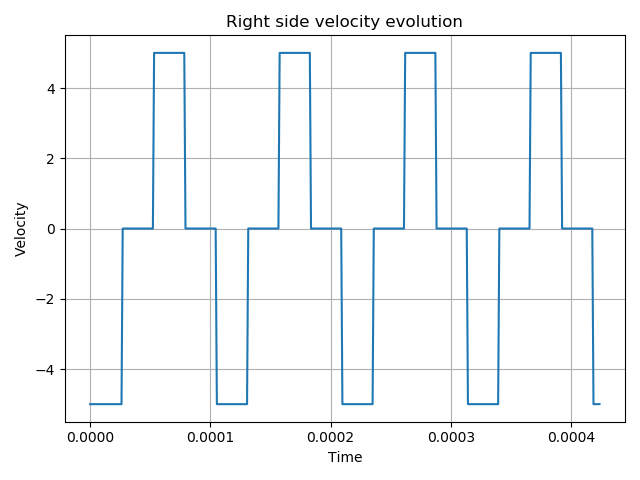
\includegraphics[width=\columnwidth]{Figures/1D_right_Velocity.png}
  }
  \caption[Velocities values in the right side of the Dyka
  bar]{Analytical solution for the velocity in the right side of the Dyka bar.}
  \label{fig:vel_analytics_dyka}
\end{figure}

\begin{figure}\sidecaption
  \centering
  \resizebox{\hsize}{!}{
    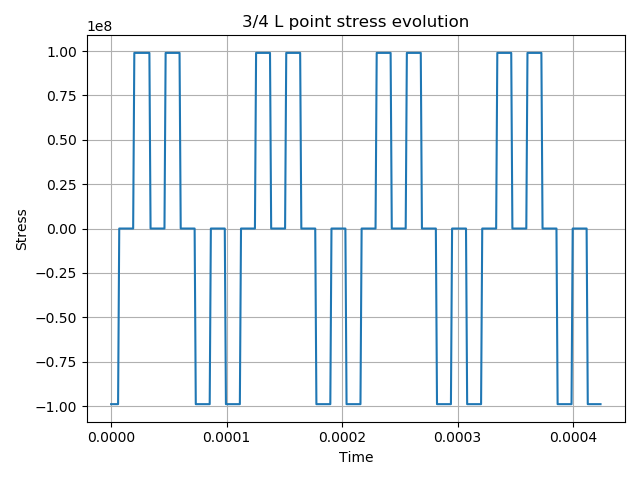
\includegraphics[width=\columnwidth]{Figures/1D_left_Stress.png}
  }
  \caption[Stress values in the last quarter side of the Dyka
  bar]{Analytical solution for the stress in the last quarter of the Dyka bar.}
  \label{fig:stress_analytics_dyka}
\end{figure}


%%%%%%%%%%%%%%%%%%%%%%%%%%%%%%
% name your BibTeX data base
\bibliography{Biblio/Biblio}
\end{document}
%%%%%%%%%%%%%%%%%%%%%%%%%%%%%%


%%% Local Variables:
%%% mode: latex
%%% TeX-master: t
%%% End: